\documentclass[pdflatex,sn-basic]{sn-jnl}

\usepackage{graphicx}%
\usepackage{multirow}%
\usepackage{amsmath,amssymb,amsfonts}%
\usepackage{amsthm}%
\usepackage{mathrsfs}%
\usepackage[title]{appendix}%
\usepackage{xcolor}%
\usepackage{textcomp}%
\usepackage{manyfoot}%
\usepackage{booktabs}%
\usepackage{algorithm}%
\usepackage{algorithmicx}%
\usepackage{algpseudocode}%
\usepackage{listings}%
\usepackage{bm}%
\usepackage{float}%
\geometry{margin=2.2cm}%

\newcommand{\R}{\mathbb{R}}
\newcommand{\bfa}{\bm{a}}
\newcommand{\bfc}{\bm{c}}
\newcommand{\bfPhi}{\bm{\Phi}}
\newcommand{\bfSigma}{\bm{\Sigma}}
\newcommand{\bfTheta}{\bm{\Theta}}
\newcommand{\bfxi}{\bm{\xi}}
\newcommand{\bfu}{\bm{u}}
\newcommand{\norm}[1]{\left\|#1\right\|}

\theoremstyle{thmstyleone}%
\newtheorem{theorem}{Theorem}%
\newtheorem{proposition}[theorem]{Proposition}%
\theoremstyle{thmstyletwo}%
\newtheorem{example}{Example}%
\newtheorem{remark}{Remark}%
\theoremstyle{thmstylethree}%
\newtheorem{definition}{Definition}%

\raggedbottom

\begin{document}

\title[Interpretable ROM for near-wall turbulence]{An interpretable reduced-order model for real-time estimation of
near-wall turbulence}

\author*[1]{\fnm{M.} \sur{P\'{e}rez Cuadrado}}\email{miguel.perez-cuadrado@citystgeorges.ac.uk}

\author[1]{\fnm{G.M.} \sur{Cavallazzi}}%\email{Giorgio.Cavallazzi@citystgeorges.ac.uk}

\author[2]{\fnm{A.} \sur{Nóvoa}}%\email{a.novoa@imperial.ac.uk}

\author[1]{\fnm{A.} \sur{Pinelli}}%\email{Alfredo.Pinelli.1@citystgeorges.ac.uk}

\affil*[1]{\orgdiv{Department of Engineering, School of Science and
Technology}, \orgname{City St George's, University of London},
\orgaddress{\city{London}, \country{UK}}}

\affil*[2]{\orgdiv{ Department of Aeronautics}, \orgname{Imperial College London},
\orgaddress{\city{South Kensington Campus,London, SW7 2BX}, \country{UK}}}

\abstract{The near-wall region of a turbulent flow maintains a self-sustaining cycle
of streaks and quasi-streamwise vortices, and this cycle leaves an uneven footprint on
the wall shear stress. Whether its dynamics, and not merely a snapshot, can be
recovered from the wall shear alone is the question addressed here. A reduced-order
model is fitted directly in the wall-shear coordinates: the trajectory is resampled
uniformly in arc length to drive the empirical measure towards the physical one, the
states are clustered under a local Mahalanobis metric adapted to the attractor's
geometry, and a single global regression over radial basis functions gives a
differentiable latent vector field. Applied to a minimal turbulent channel at friction
Reynolds number 180, the geometry-adapted clustering separates the mature-streak,
breakdown and quiescent phases into sharp populations that map onto the known
coherent-structure skeleton, without physical labels. Integrated freely, the model
stays bounded and reproduces the invariant measure; being differentiable, it locates
the cycle's weakly unstable near-equilibria and resolves its non-normal growth and
phase-volume contraction by phase. An ensemble Kalman filter assimilating sparse,
noisy wall measurements tracks the true trajectory and gauges how far the instantaneous
wall shear determines the cycle: the model holds the climate, and the forecast error it
incurs from the unobserved interior motions is bounded and concentrated in the active
phase.}

\keywords{wall turbulence, reduced-order modelling, sparse identification of
nonlinear dynamics, radial basis functions, Mahalanobis metric,
invariant measure}

\maketitle

\section{Introduction}\label{sec:intro}
The dynamics of near-wall turbulence are organised around a self-sustaining
cycle \citep{Waleffe_1997}. Within this cycle, elongated low-speed streaks form
by lift-up \citep{brandt2014liftup}, undergo a sinuous instability, break down
\citep{andersson2001breakdown}, and regenerate over a characteristic time of
about a hundred wall units \citep{Hamilton_Kim_Waleffe_1995}. The cycle is
spatially compact, confined to a minimal flow unit \citep{jimenez1991minimal},
and it remains autonomous when the outer flow is removed
\citep{jimenez1999autonomous}.

The discovery of this cycle motivated strategies to control it. These strategies
are based on sensing the velocity close to the wall and acting on the wall to
break the cycle and reduce drag, ranging from opposition control
\citep{choi1994active} to machine-learned policies
\citep{guastoni2023drl,cavallazzi2025drl}. However, sensing at that wall-normal
distance requires reaching into the flow above the wall, which is impractical in
experiment and at high Reynolds number, whereas the shear stress at the wall
itself is directly measurable \citep{naughton2002modern,lofdahl1999mems}. The
question becomes whether the cycle can be recovered from wall variables alone.

Recovering the signature of the near-wall structures from the wall has been
approached in several settings, mainly wall modelling
\citep{piomelli2002walllayer,bose2018wallmodeled}. Near-wall coherent motions
\citep{robinson1991coherent} leave a footprint on the wall, in the pressure
\citep{naguib2001stochastic} and in the shear stress
\citep{kravchenko1993relation}, so the near-wall field is observable from wall
quantities alone and can be reconstructed instantaneously
\citep{guemes2021coarse,cuellar2024threedimensional}. Larger structures further
from the wall can be sensed too, provided they remain attached
\citep{encinar2019logarithmic}.

This footprint is uneven across the cycle, however: the wall-attached streaks
leave a strong, direct signature in the streamwise shear
\citep{robinson1991coherent}, whereas the quasi-streamwise vortices of the
breakdown and regeneration phase register only indirectly, through their imprint
on the spanwise shear, which at the wall is the exact footprint of the near-wall
streamwise vorticity, $\tau_y = \mu\,\omega_x$. An instantaneous reconstruction
is a snapshot, though, not the cycle. Recovering the cycle's dynamics, and so
testing whether the wall retrieves it at all, needs more than a snapshot: a model
that advances the wall state on its own, staying bounded and reproducing the
correct statistics under free integration.

Modelling such dynamics from data is a task that can be handed to a reduced-order
model, which compresses the flow into a few latent coordinates, far below the
dimension of the underlying direct numerical simulation, and advances them in
time. Such models are either intrusive or non-intrusive \citep{benner2015survey}.

Intrusive models use knowledge of the governing equations, projecting them onto
the latent space. POD--Galerkin models are the canonical example: proper
orthogonal decomposition \citep{lumley1967structure,sirovich1987turbulence}
supplies the compression, and the Navier--Stokes equations are projected onto the
retained modes, globally \citep{Cavalieri_Nogueira_2022} or on locally defined
bases \citep{colanera2025qlrom,Colanera_MFU}. Since the truncated small scales
drain energy from the retained modes, such projections are prone to instability
\citep{rempfer2000low}, and the discarded scales must be reintroduced through a
calibrated eddy-viscosity dissipation to recover stable long-time statistics
\citep{Aubry_Holmes_Lumley_Stone_1988}.

Non-intrusive models instead learn the reduced dynamics directly from data,
absorbing the truncation effect implicitly and requiring no access to the
governing operator. Some remain opaque, such as recurrent networks that predict
accurately but act as black boxes \citep{Srinivasan_NN_MFU}; others are
interpretable, such as sparse symbolic regression \citep{brunton2016discovering}
or cluster-based networks of coherent states
\citep{kaiser2014cluster,fernex2021cluster}.

For the minimal channel, though, these models sit on one side of what is needed or
the other. The reconstructions take the wall as input but carry no dynamics,
returning only the instantaneous field \citep{guastoni2021convolutional}; the
reduced-order models that do carry the dynamics are built on the full field, not
on the wall \citep{nakamura2021convolutional}. A reduced-order model of the
dynamics from the wall alone, which is what testing the cycle's
wall-recoverability asks for, does not yet exist.

Data assimilation bridges the two by folding measurements into a running model:
an ensemble Kalman
filter corrects the forecast towards partial, noisy observations of the
full-order flow. \citet{colburn2011state} did so for a turbulent channel with
the governing equations in the loop, and \citet{ozalp2026realtime} with a
data-driven reduced-order model in their place. The same filter has two uses:
it pulls the model towards the true trajectory, and the mismatch between its
forecast and the observations measures how much correction the model needs to
stay consistent with the data \citep{desroziers2005diagnosis,anderson2007adaptive}.

We propose to test whether the wall closes the near-wall cycle as a dynamical
object, using the reduced-order model of \citet{perezcuadrado2026manifold}, whose
machinery is taken as established and applied to a minimal turbulent channel
\citep{jimenez1991minimal} at friction Reynolds number $Re_\tau = 180$
\citep{kim1987turbulence}. The observable is the wall shear stress alone, which is
the direct footprint of the near-wall velocity gradient and whose two components
record the streaks and the quasi-streamwise vortices; the non-local wall pressure
is left aside. The field is compressed by proper orthogonal
decomposition, and its reduced coordinates are advanced by a vector field fitted
to the data, without the governing equations.

This combination is new. Prior wall-based estimators are either intrusive, tied
to the governing equations \citep{colburn2011state}, or rest on opaque
data-driven models \citep{ozalp2026realtime}, whereas the present model is
non-intrusive, interpretable, and preserves the invariant measure of the wall
shear \citep{vlachas2020}. Measure preservation also aids the assimilation: a
model that stays on the attractor gives the filter a physically consistent
forecast covariance \citep{evensen2003ensemble,dee1995online}, where a drifting
model would report the wrong one.

Three results follow. Clustering the wall-shear trajectory recovers the
coherent-structure skeleton: its phases fall onto the streak--vortex plane as a
directed cycle, from the quiescent state through the vortex-dominated state to the
mature streak, and the field fitted on this partition reproduces the invariant
measure of the skin friction under free integration. Read as a dynamical system,
that field places its slow points only in the quiescent phase and amplifies perturbations
most as the streak matures towards breakdown. The ensemble Kalman filter
then measures how complete the wall-only description is: the additive inflation
needed to keep its forecast consistent with sparse, noisy wall sensors is the
price, in inflation units, of the interior variability the wall cannot carry. The
wall shear reproduces the cycle's statistics on its own but not its trajectory, a
statistical rather than deterministic autonomy of the cycle in the wall
observable.

\section{Modelling pipeline}\label{sec:pipeline}
The model advances the wall shear stress in a latent space, following the
reduced-order pipeline introduced by \citet{perezcuadrado2026manifold}, which we
reproduce in Fig.~\ref{fig:pipeline} for reference. At each instant the two wall
shear-stress components are encoded by proper orthogonal decomposition into a
small set of latent coordinates. A vector field, fitted once to the data, advances
those coordinates in time, and the decoder maps them back to the wall shear-stress
fluctuation. The vector field is built from a radial-basis library whose centres
respect the geometry of the attractor rather than the variance hierarchy of the
decomposition.

\begin{figure}[H]
	\centering
	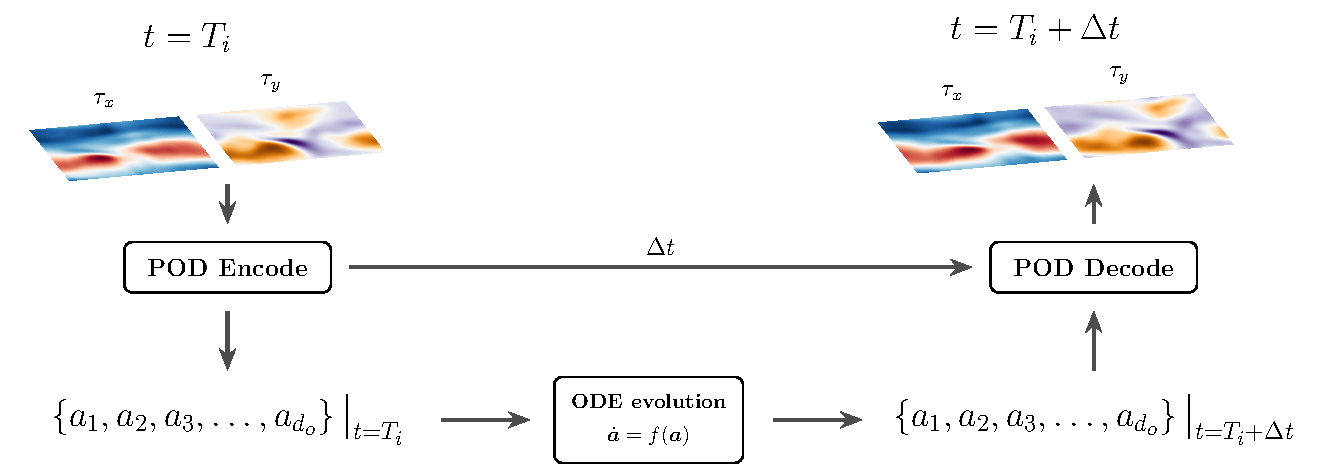
\includegraphics[width=\textwidth]{images/fig1_planes3d.pdf}
	\caption{Modelling pipeline. The wall shear-stress components
	$(\tau_x,\tau_y)$ at time $T_i$ are encoded onto latent coordinates by
	proper orthogonal decomposition, advanced by the learned sparse vector
	field $\dot{\bfa}=f(\bfa)$, and decoded back to the wall shear-stress
	fluctuation at $T_i+\Delta t$.}
	\label{fig:pipeline}
\end{figure}

The remainder of the paper follows this chain. Section~\ref{sec:flow} describes
the channel simulation and the proper orthogonal decomposition of the wall shear.
The latent trajectory is then clustered, and the resulting partition is shown to
recover the coherent-structure skeleton of the near-wall cycle
(Section~\ref{sec:dynstates}). On the corrected geometry the sparse vector field is
fitted and integrated in free running to test its invariant measure and
predictability horizon (Section~\ref{sec:recover}). The fitted field, explicit and
differentiable, is then read as a dynamical system, giving the cycle's slow points
and the ordering of non-normal growth around the burst (Section~\ref{sec:interp}). Sparse and noisy wall observations are finally
folded back into the running model with an ensemble Kalman filter, whose required
inflation bounds the interior variability the wall does not carry
(Section~\ref{sec:enkf}).

\section{Flow configuration and the wall observable}\label{sec:flow}
The wall shear stress that the model advances is produced by direct numerical
simulation of a turbulent channel flow at friction Reynolds number $Re_\tau = 180$,
computed with the solver CaNS \citep{costa2018fft}, which integrates the
incompressible Navier--Stokes equations on a staggered grid by second-order finite
differences in space, a low-storage three-stage Runge--Kutta scheme in time and a
pressure-correction step that enforces continuity at each substep, with the flow held at
constant mass flow rate.

The domain follows the minimal channel introduced by
\citet{jimenez1991minimal}, a half-channel of streamwise, spanwise and
wall-normal extent $480^+ \times 140^+ \times 180^+$, closed by a symmetry
condition at the midplane. The wall-parallel plane is resolved by $64 \times 64$
points, giving spacings $\Delta x^+ \approx 7.5$ in the streamwise and
$\Delta y^+ \approx 2.2$ in the spanwise direction, while the wall-normal
direction is stretched, its near-wall spacing decreasing to
$\Delta z^+ = 0.54$ at its minimum. This resolution is consistent with established
near-wall channel simulation \citep{kim1987turbulence}. Integration proceeds
at a fixed step $\Delta t = 0.01$, and the two wall shear-stress components, the
streamwise $\tau_x$ and the spanwise $\tau_y$, are recorded every five steps, about
half a wall time unit apart.

This interval is set by the accuracy of
the reduced description rather than by storage: it must resolve the reduced
coordinates finely enough for their time derivatives, which the model targets, to
be estimated smoothly and for the projected coefficients to be well resolved in
time. Sampling continues to $10^5$ snapshots, spanning roughly $5 \times 10^4$
wall time units.

At each instant the two components
$(\tau_x,\tau_y)$ are stacked into a single vector $\bfu\in\R^{N}$ of dimension
$N = 2\times 64\times 64 = 8192$. The $M = 10^5$ recorded fields are reduced by
proper orthogonal decomposition \citep{lumley1967structure,sirovich1987turbulence}. The temporal
mean is removed first, so that the
basis describes the fluctuations about the mean wall state,
\begin{equation}
	\bar{\bfu} = \frac{1}{M}\sum_{m=1}^{M}\bfu_m, \qquad
	\bfu'_m = \bfu_m - \bar{\bfu}.
	\label{eq:fluct}
\end{equation}
Collecting the centred fields as the columns of a snapshot matrix and taking its
singular value decomposition, the equations
\begin{equation}
	\mathbf{X} = [\,\bfu'_1,\dots,\bfu'_M\,]\in\R^{N\times M}
	\quad\text{and}\quad
	\mathbf{X} = \bfPhi\,\bfSigma\,\bm{\Psi}^{\top}
	\label{eq:svd}
\end{equation}
give the proper orthogonal modes as the columns of $\bfPhi$, an orthonormal
basis ordered by the singular values on the diagonal of $\bfSigma$, whose squares
measure the fluctuation energy carried by each mode. Retaining the leading $d_o$
modes $\bfPhi_{d_o}$, the reduced coordinates and the reconstruction of the wall
field are
\begin{equation}
	\bfa(t) = \bfPhi_{d_o}^{\top}\big(\bfu(t)-\bar{\bfu}\big)\in\R^{d_o},
	\qquad
	\bfu(t)\approx\bar{\bfu} + \bfPhi_{d_o}\,\bfa(t),
	\label{eq:reduced}
\end{equation}
and the projection of each snapshot gives the reduced trajectory
$\bfa_m = \bfPhi_{d_o}^{\top}\bfu'_m$ on which the model operates.

\begin{figure}[H]
	\centering
	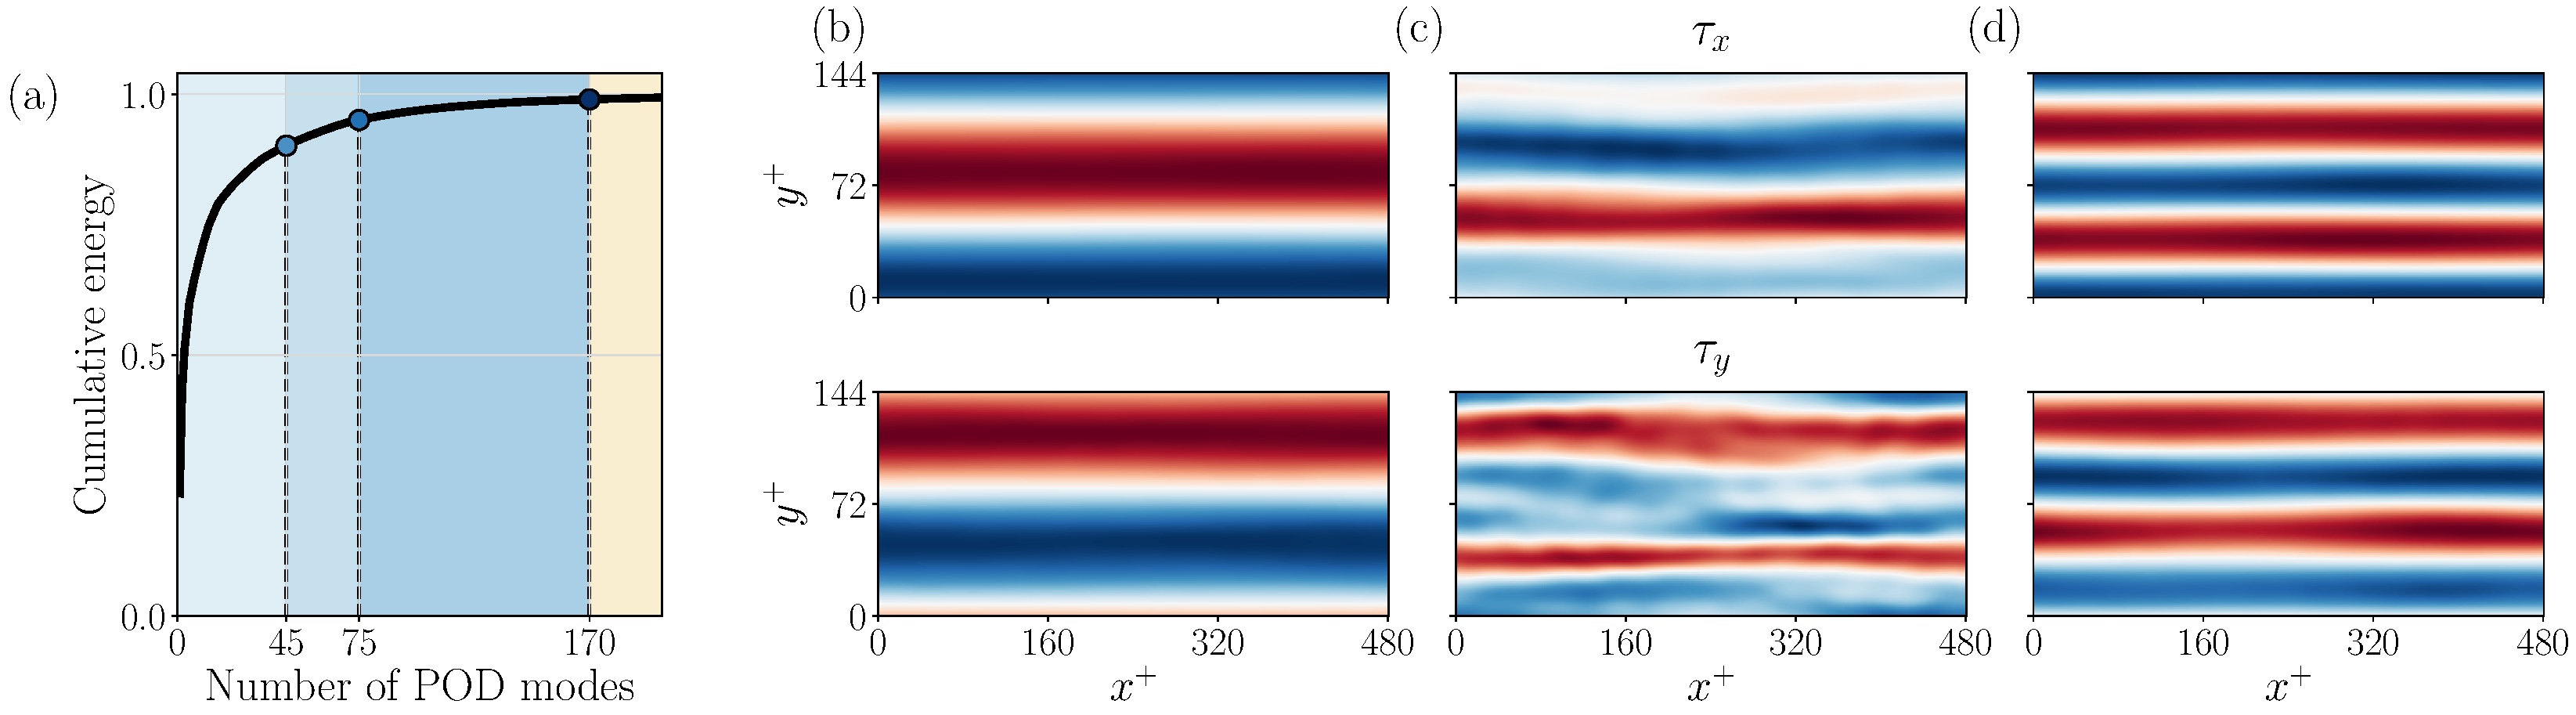
\includegraphics[width=\textwidth]{images/fig2_reduction_grid.pdf}
	\caption{Proper orthogonal decomposition of the wall shear stress.
	(a) Cumulative fluctuation energy against the number of retained modes,
	with the $90\%$, $95\%$ and $99\%$ thresholds reached at $d_o = 45$, $75$
	and $170$ modes. (b--d) Streamwise $\tau_x$ (top row) and spanwise $\tau_y$
	(bottom row) components of proper orthogonal modes 2, 4 and 6}
	\label{fig:reduction}
\end{figure}

The model operates on the leading $d_o = 45$ modes, which carry about $90\%$ of
the fluctuation energy (Fig.~\ref{fig:reduction}a). The discarded tail is
dominated by small-scale, low-energy wall-gradient content, so the operating
dimension follows the dynamically relevant scales rather than the reconstruction
accuracy alone. That $d_o = 45$ carries the cycle's dynamics is borne out by the
free-run climate of Section~\ref{sec:recover}, where the modes added up to $d_o = 75$
leave the recovered statistics unchanged; the clustering diagnostics of
Section~\ref{sec:dynstates} independently share the same elbow at $d_o = 45$, $75$ and
$170$. These higher-dimensional truncations are carried alongside for comparison.

The leading modes carry the wall imprint of the near-wall streaks; the streamwise
and spanwise components of mode 2 are shown in Fig.~\ref{fig:reduction}(b). Modes 1
and 2 form a symmetric pair, and together they span the streak over its spanwise
phase. This is consistent with velocity-field proper orthogonal decompositions of
channel turbulence \citep{moin1989characteristic,Aubry_Holmes_Lumley_Stone_1988},
whose wall imprint the shear-stress decomposition inherits.

The model requires the reduced coordinates together with their time derivatives.
The derivatives are obtained by numerical differentiation of the coordinate time
series, a five-point finite-difference stencil accurate to fourth order in the
sampling interval \citep{brunton2016discovering}. Finite differencing amplifies
high-frequency noise, but the retained coordinates are smooth, the small-scale
tail having been truncated, so noise-resistant differentiation
\citep{chartrand2011numerical} is not required. Each snapshot then carries the
reduced state and its velocity as a pair $(\bfa_m,\dot{\bfa}_m)$, and this set of
pairs is the data from which the reduced dynamics are fitted.

\section{Dynamical states via unsupervised clustering}\label{sec:dynstates}

The latent trajectory is partitioned into clusters, each adapting the shape of its
radial basis functions to the local geometry of the manifold
\citep{perezcuadrado2026manifold}. The number of clusters is judged by the
separation it draws between neighbouring regions of the attractor, measured by three
diagnostics: the marginal Bayesian information criterion \citep{schwarz1978estimating} $\Delta\mathrm{BIC}/\Delta K$
(Fig.~\ref{fig:clusterK}(a)), the shape difference between neighbours $|P_i - P_j|$
(Fig.~\ref{fig:clusterK}(b)), and the relative speed gap $|v_i - v_j|/(v_i + v_j)$
(Fig.~\ref{fig:clusterK}(c)).

Beyond $K = 16$ all three truncations level off, oscillating about the same range.
The final values of the three metrics differ between $d_o = 45$, $75$ and $170$, but the curves share the same
shape and the same elbow, a first indication that $d_o = 45$ already carries the skeleton of
the dynamical system.

\begin{figure}[H]
	\centering
	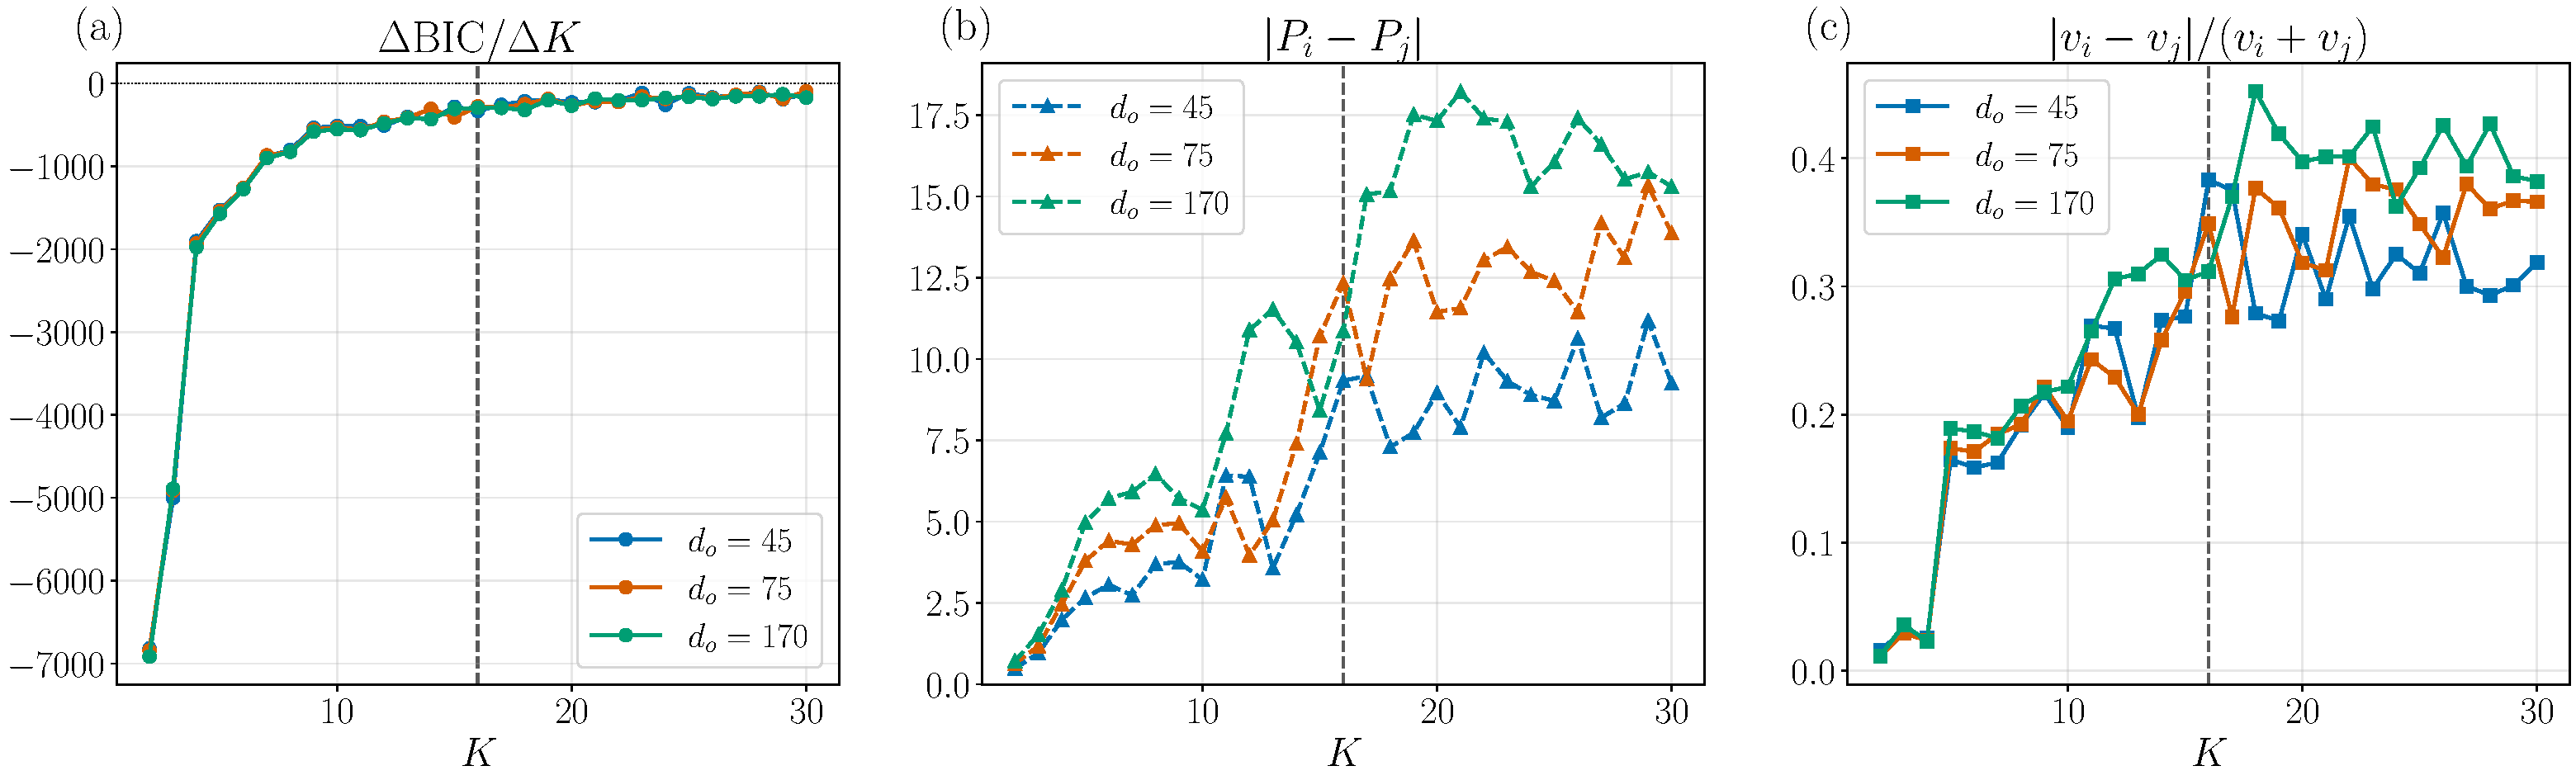
\includegraphics[width=\textwidth]{images/fig3_cluster_metrics_all.pdf}
	\caption{Selecting the number of clusters. Three separation diagnostics
	against the number of clusters $K$, each for $d_o = 45$, $75$ and $170$,
	with the chosen $K = 16$ marked by the dashed line: (a) the marginal Bayesian
	information criterion $\Delta\mathrm{BIC}/\Delta K$; (b) the
	participation-ratio gap $|P_i - P_j|$ between neighbouring clusters;
	(c) the relative speed gap $|v_i - v_j|/(v_i + v_j)$.}
	\label{fig:clusterK}
\end{figure}

These diagnostics fix the number of clusters but not their meaning. Whether the sixteen
clusters mark stages of the known wall cycle or merely cut the attractor into unconnected
regions is settled by the cycle itself. If each phase is a distinct physical event,
the wall signature of each cluster should carry information about the stage it represents.
Since the expected alternation is between
streaks and quasi-streamwise vortices, we look for the distinct scalar footprint each leaves on the wall.

The streaks are streamwise-elongated, spanwise-alternating modulations of the
streamwise velocity \citep{robinson1991coherent}, so $\tau_x$ is the natural streak marker.
The streak intensity is the streamwise-averaged, $k_y=1$ Fourier amplitude of the reconstructed
fluctuation,
\begin{equation}
	A_x = \frac{1}{\tau_w}\,
	\big|\,\widehat{\langle\tau_x'\rangle_x}\,(k_y{=}1)\,\big|,
	\label{eq:streak}
\end{equation}
with $\tau_w$ the mean wall shear, $\langle\cdot\rangle_x$ the streamwise average
and the hat the spanwise Fourier transform. The streamwise average sets
$k_x{=}0$, and the fundamental spanwise mode $k_y{=}1$ isolates the
single-wavelength streak. This wall-shear amplitude is the analogue
of the fundamental-spanwise-mode streak measure of \citet{Hamilton_Kim_Waleffe_1995}.

The vortices leave their mark on the
spanwise shear instead: at the wall the spanwise shear is the exact footprint of
the near-wall streamwise vorticity, $\tau_y = \mu\,\omega_x$, so its strength
measures the vortices directly.
The vortex strength is taken as the root-mean-square of that fluctuation over the wall plane,
\begin{equation}
	\sigma_y = \frac{1}{\tau_w}\,
	\big\langle \tau_y'^{\,2} \big\rangle^{1/2}.
	\label{eq:qsv}
\end{equation}
The two markers place each wall field on the streak--vortex plane
$(A_x,\sigma_y)$, where the cycle's alternation between streak formation and
vortex regeneration should appear as an orbit and each cluster as one of its
phases.

The cluster-averaged markers (standardised to zero mean and unit variance) are shown in
Fig.~\ref{fig:phasecycle}(a),
together with the dominant transitions between clusters.
The occupied quadrants mark three phases of the regeneration
cycle \citep{Hamilton_Kim_Waleffe_1995,Waleffe_1997}:
the quiescent state, low $A_x$ and low $\sigma_y$, in Q3;
the mature high-amplitude streak in Q1;
and the vortex-dominated state, $\sigma_y$ high with the coherent streak still weak, in Q2.
This interpretation is coherent with the cluster-averaged $\tau_x$ fields
in Fig.~\ref{fig:phasecycle}(d--f):
Q1 carries a strong, streamwise-coherent low-speed streak;
Q2 the same bands with their streamwise coherence reduced, modulated along the
streamwise direction and pinched into closed $\tau_x$ contours;
and Q3 a weak, low-amplitude remnant of the streak.

The partition used no physical labels, yet its centroids fall onto the three phases of the
near-wall cycle once read through the wall markers, each phase in a cluster of its own. The
separation follows from the manifold-adapted clustering of \citet{perezcuadrado2026manifold},
which corrects the coordinate and sampling biases that would otherwise blur the phases together.

The transitions between these phases carry a directed sense,
made visible in Fig.~\ref{fig:phasecycle}(b) by high-pass filtering the two markers
and rendering their mean phase velocity as streamlines.
The spanwise shear leads the streak by about $13\,t^+$, roughly a tenth of the cycle,
so the circulation is clockwise, the vortices rising ahead of the coherent streak
before both markers relax towards the quiescent Q3, the order consistent with
lift-up \citep{brandt2014liftup}.

The circulation is not a causality claim. Built from wall footprints, it is
the kinematic skeleton of the wall-projected dynamics, the phases and the sense in which
they succeed one another rather than the drive behind them. On a closed cycle a phase lead
marks position, not drive, so the observed lift-up sense need not follow the causal arrow;
the dominant causal direction found by \citet{lozanoduran2020causality} in fact runs the
other way, the streak instability regenerating the vortices. The wall thus returns the
cycle's directed skeleton, not the mechanism that drives it.
\begin{figure}[H]
	\centering
	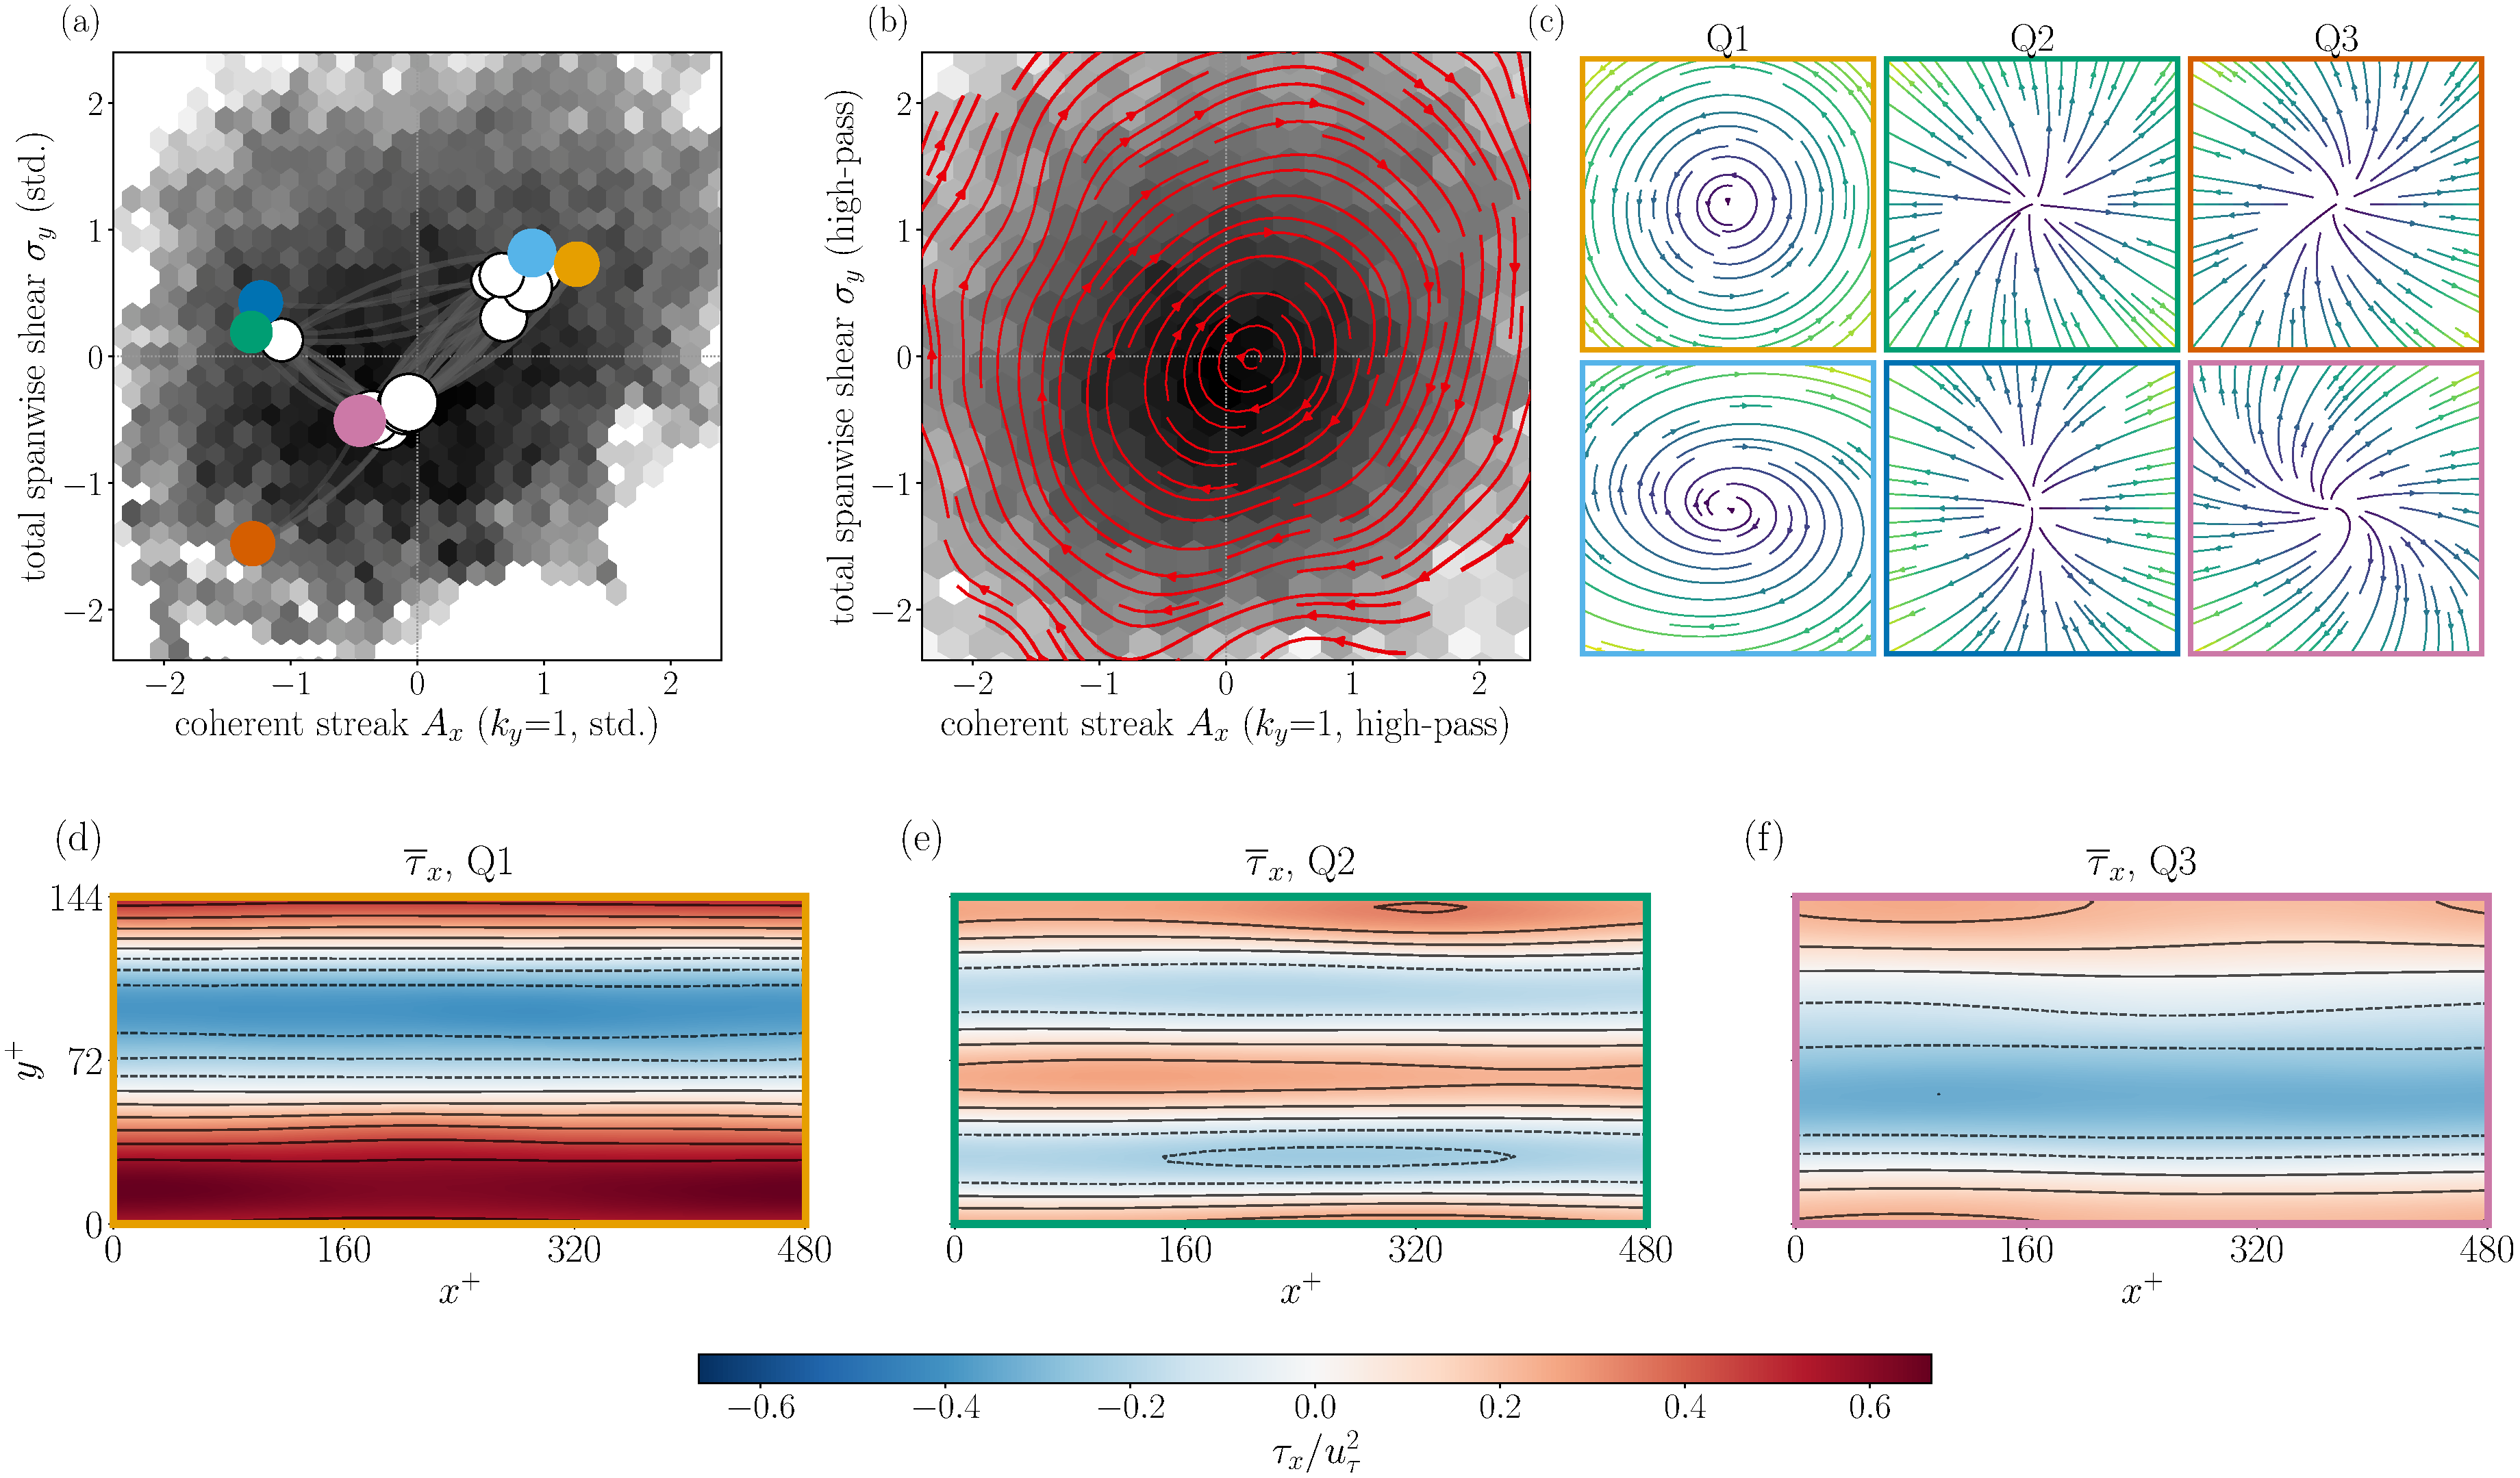
\includegraphics[width=\textwidth]{images/fig4_phase_cycle.pdf}
	\caption{The near-wall cycle on the streak--vortex plane. (a,b) Plane
	spanned by the coherent streak amplitude $A_x$, the $k_y = 1$ spanwise
	fundamental of $\tau_x'$, and the spanwise-shear intensity $\sigma_y$.
	(a) The sixteen
	cluster centroids on the standardised plane, sized by occupancy, over the
	sampled density (grey), with arrows for the dominant inter-cluster
	transitions. (b) The same plane after high-pass filtering, with red
	streamlines of the mean phase velocity; the winding directedness
	$D = \overline{\dot\theta}/\overline{|\dot\theta|} = -0.20$ gives a weak but
	significant clockwise circulation. (c) Local dynamics of the fitted field,
	the leading-plane projection of the Jacobian $J_k$ at two clusters per
	quadrant, streamlines shaded by the local rate; 
	Border colours link each tile to its cluster in (a). (d--f)
	Cluster-averaged streamwise shear $\overline{\tau}_x$ of the representative
	cluster in Q1, Q2 and Q3: the mature streak, its loss of coherence, and the
	quiescent state.}
	\label{fig:phasecycle}
\end{figure}

The clusters fall on the cycle's phases, but position is not dynamics: a partition can carve
a continuous attractor into pieces that sit apart yet behave alike. Clustering is justified
only where the local dynamics, not the position alone, separate the phases
\citep{perezcuadrado2026manifold}. Being differentiable, the fitted field lets this be checked
at each cluster's centroid: linearising it there gives the Jacobian $J_k$, which reads out how the
trajectories passing through the cluster are deformed.

At each centroid the leading eigenvalue of $J_k$ has positive real part, so the leading
direction expands and pushes nearby trajectories apart. The character of that eigenpair sets the
phases apart (Fig.~\ref{fig:phasecycle}c): the mature streaks of Q1 are complex-dominant,
a rotational deformation of neighbouring trajectories; the Q2 clusters largely real-dominant,
straining them without rotation; Q3 lies between.
This split confirms that the clusters isolate dynamically distinct stages of the cycle.
Where cluster-based reduced-order models represent the phase dynamics
by transition probabilities between clusters \citep{kaiser2014cluster,fernex2021cluster},
the differentiable field here lets each phase be read instead as a local deformation.




\section{Model fitting and free integration}\label{sec:recover}
After clustering and adapting the RBFs to the local geometry \citep{perezcuadrado2026manifold},
the model is fitted by a single sparse regression over the
radial basis functions, giving the vector field $\dot{\bfa} = f(\bfa)$. The record is split in
time, the first $80\%$ used for the regression and the final $20\%$ held out to test it.

Two
parameters of the library are left free: the number of basis functions $N$ and the tangent
anisotropy $\alpha_{\mathrm{tan}}$, which scales the width of every kernel along the local
manifold tangent by a single common factor. The fit is studied at two truncations, $d_o=45$ and $75$.
The modes beyond these are small-scale wall-gradient fluctuations, incoherent with the streaks
and quasi-streamwise vortices that carry the cycle
\citep{jimenez1991minimal,Hamilton_Kim_Waleffe_1995,Waleffe_1997}, so the $99\%$-energy
truncation $d_o=170$ of Section~\ref{sec:dynstates} is not carried into the dynamical model.
Both parameters are swept for $d_o=45$ and $75$ (Fig.~\ref{fig:alphanrmse}a,b); the error
shown is the test NRMSE, normalised per mode by that mode's test-segment standard deviation and
averaged over the retained modes.

At small $\alpha_{\mathrm{tan}}$ the kernels are narrower than the
spacing between their centres and their supports leave gaps across the manifold; coverage then
improves only slowly with $N$, and at the smallest widths no number of kernels within the swept
range fills the space, so the error stays near unity. As $\alpha_{\mathrm{tan}}$ grows the supports overlap, the
manifold is covered, and the error decreases. Once the width is sufficient each curve reaches a
minimum at an intermediate $N$ and rises beyond it, the fit passing from under-parameterised to
over-parameterised as the extra kernels begin to follow noise; the larger the width, the fewer
kernels needed to reach that point.

The floor of each curve, its lowest error over $N$, is shown against $\alpha_{\mathrm{tan}}$
in Fig.~\ref{fig:alphanrmse}(c), where the two truncations cross. At small
$\alpha_{\mathrm{tan}}$ the lower-dimensional model reaches the lower floor: with fewer modes
the spread of characteristic scales across dimensions is narrower, so a single global
$\alpha_{\mathrm{tan}}$ fits every dimension well. Past $\alpha_{\mathrm{tan}}\approx 10$, where coverage is no longer
the constraint, the higher-dimensional model takes the lead: retaining more modes leaves less
energy in the truncated tail, and that smaller cut-off loss sets the error.

\begin{figure}[H]
	\centering
	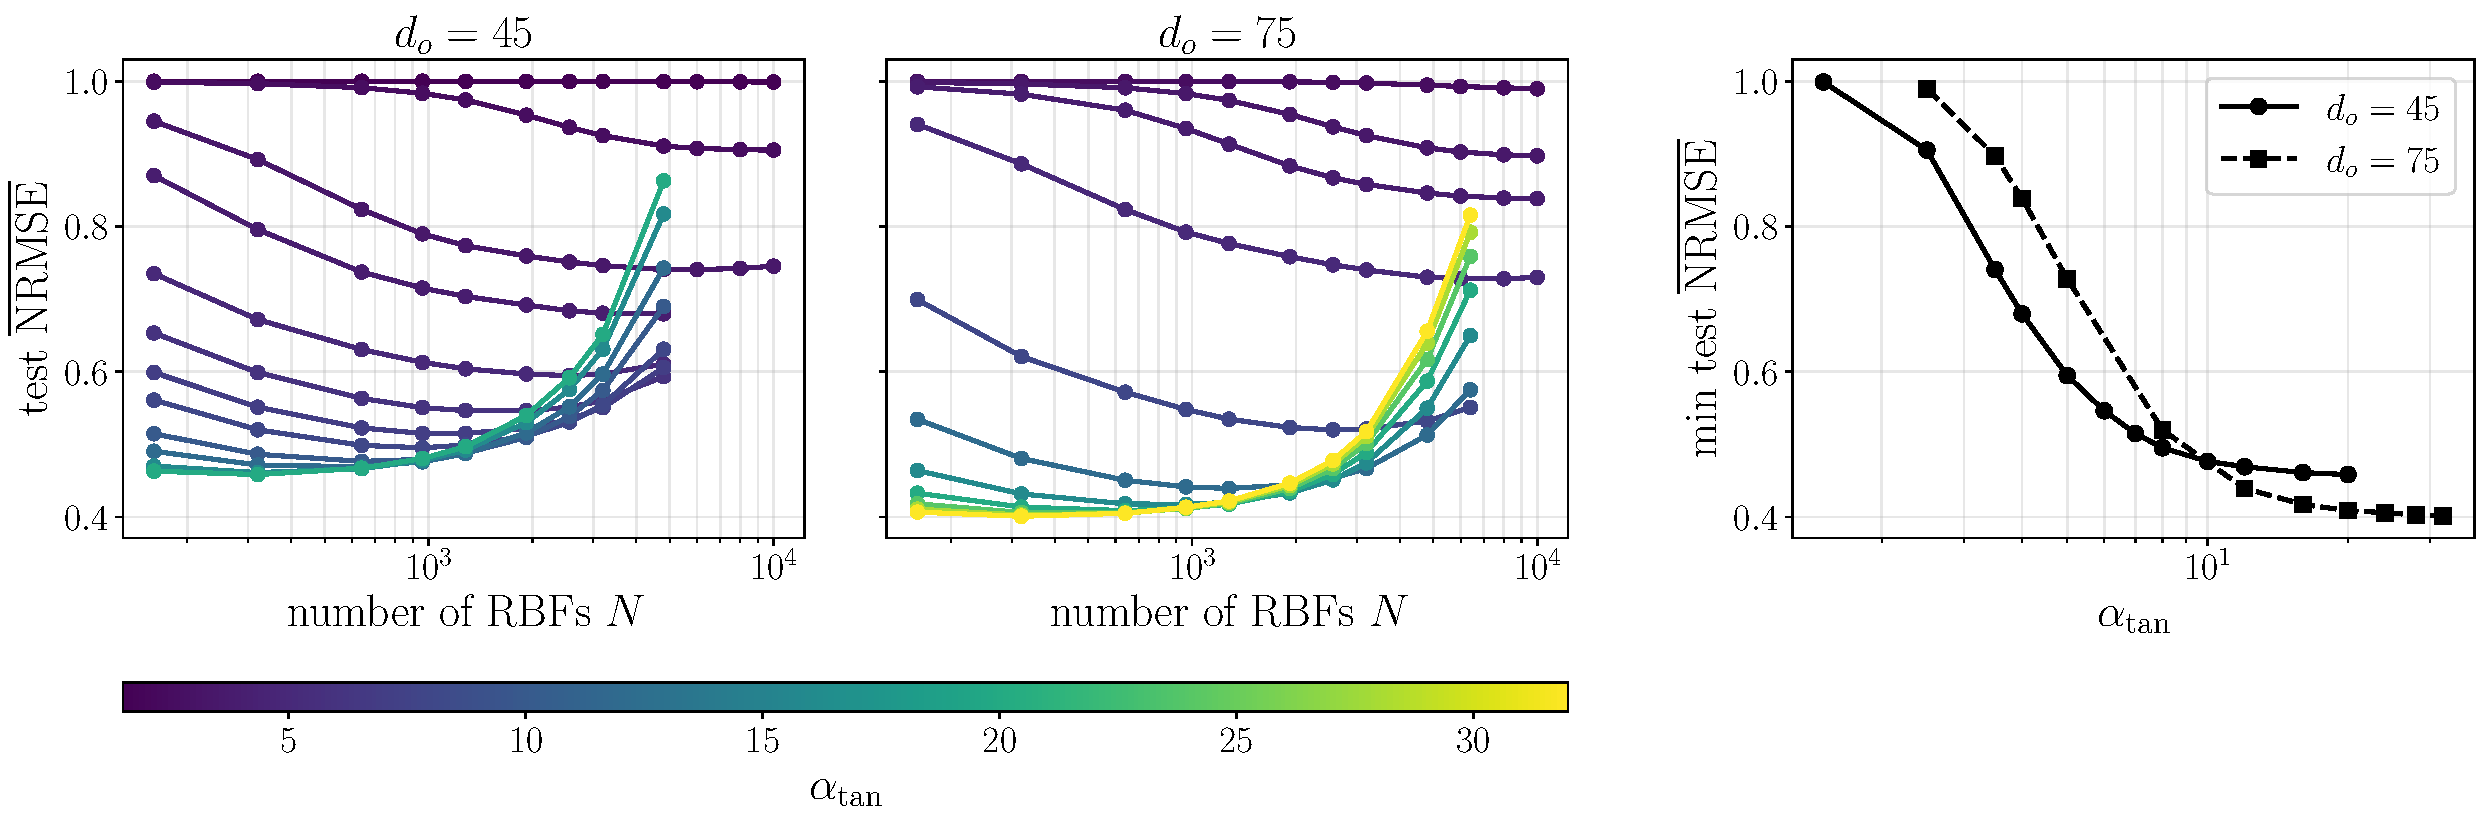
\includegraphics[width=\textwidth]{images/fig5_alpha_nrmse.pdf}
	\caption{Fitting the sparse vector field. Mode-averaged test NRMSE against the
	number of radial basis functions $N$, one curve per tangent anisotropy
	$\alpha_{\mathrm{tan}}$ (colour), for (a) $d_o=45$ and (b) $d_o=75$.
	(c) The NRMSE floor over $N$ against $\alpha_{\mathrm{tan}}$.}
	\label{fig:alphanrmse}
\end{figure}

With the library fixed, the fitted field is advanced by a fourth-order Runge--Kutta scheme
at the sampling step on which it was fitted, $\Delta t \approx 1.13\,t^+$, together with the
per-cluster trust-region corrector of the method paper \citep{perezcuadrado2026manifold},
calibrated as described there.
Each cluster's trust region is set to enclose the sampled attractor, so on-attractor trajectories
never trigger the corrector and the reported statistics are those of the fitted field itself; the
corrector acts only on excursions beyond the sampled data, pulling the trajectory back to keep the
run bounded. 

The free run is judged on two indicators. The first measures short-range accuracy through the
valid prediction time (VPT), a standard gauge of forecast quality \citep{vlachas2020}: how long a
forecast stays close to the reference. It is the time in $t^+$ before the reconstruction error
$e_{\mathrm{rec}}$, the latent-space error normalised by
$\sigma_A=\big(\textstyle\sum_i \mathrm{Var}(a_i)\big)^{1/2}$, the per-mode standard deviations
over the reference record summed in quadrature, first exceeds $0.25$; that is,
\begin{equation}
	\mathrm{VPT} = \min\{\, t : e_{\mathrm{rec}}(t) > 0.25 \,\},
	\qquad
	e_{\mathrm{rec}}(t) = \frac{\norm{\bfa_{\mathrm{ROM}}(t)-\bfa_{\mathrm{true}}(t)}}{\sigma_A}.
	\label{eq:vpt}
\end{equation}

The normalisation is global, by the single $\sigma_A$ rather than per mode, so the
threshold weights the energetic modes that carry the wall signature; the horizon is reported in
wall units $t^+$.

The long-time match is read from two distances between the free run and the reference, both
standard metrics for comparing distributions \citep{gibbs2002choosing}. With
$s(t)=\langle\tau_x\rangle(t)$ the instantaneous skin friction and $F$ its empirical distribution
over the free-run time series, the first is the Wasserstein-1 distance \citep{peyre2019computational},
\begin{equation}
	W_1 = \int \big|F_{\mathrm{ROM}}(s)-F_{\mathrm{FOM}}(s)\big|\,\mathrm{d}s,
	\label{eq:w1}
\end{equation}
reported normalised by the reference standard deviation $\sigma_{\mathrm{FOM}}$. The second
compares the shape of the skin-friction spectrum. Writing $\widehat{\phi}(f)$ for the
premultiplied power spectral density $f\,P(f)$ of each series, normalised to unit area over the
same resolved band $f\le f_{\max}$, above which the reference spectrum is band-limited, the two
shapes are compared by the total-variation distance between them as probability densities over
frequency \citep{gibbs2002choosing},
\begin{equation}
	\mathrm{TV} = \tfrac{1}{2}\int
	\big|\widehat{\phi}_{\mathrm{ROM}}(f)-\widehat{\phi}_{\mathrm{FOM}}(f)\big|\,\mathrm{d}f .
	\label{eq:tv}
\end{equation}
The half-factor and unit-area normalisation bound $\mathrm{TV}\in[0,1]$, zero for identical
spectral shapes and one for disjoint support; being area-normalised it measures shape alone,
complementing $W_1$. Both spectra are estimated with the same Welch parameters on a common
frequency grid, so the distance is free of binning artefacts.
\begin{figure}[H]
	\centering
	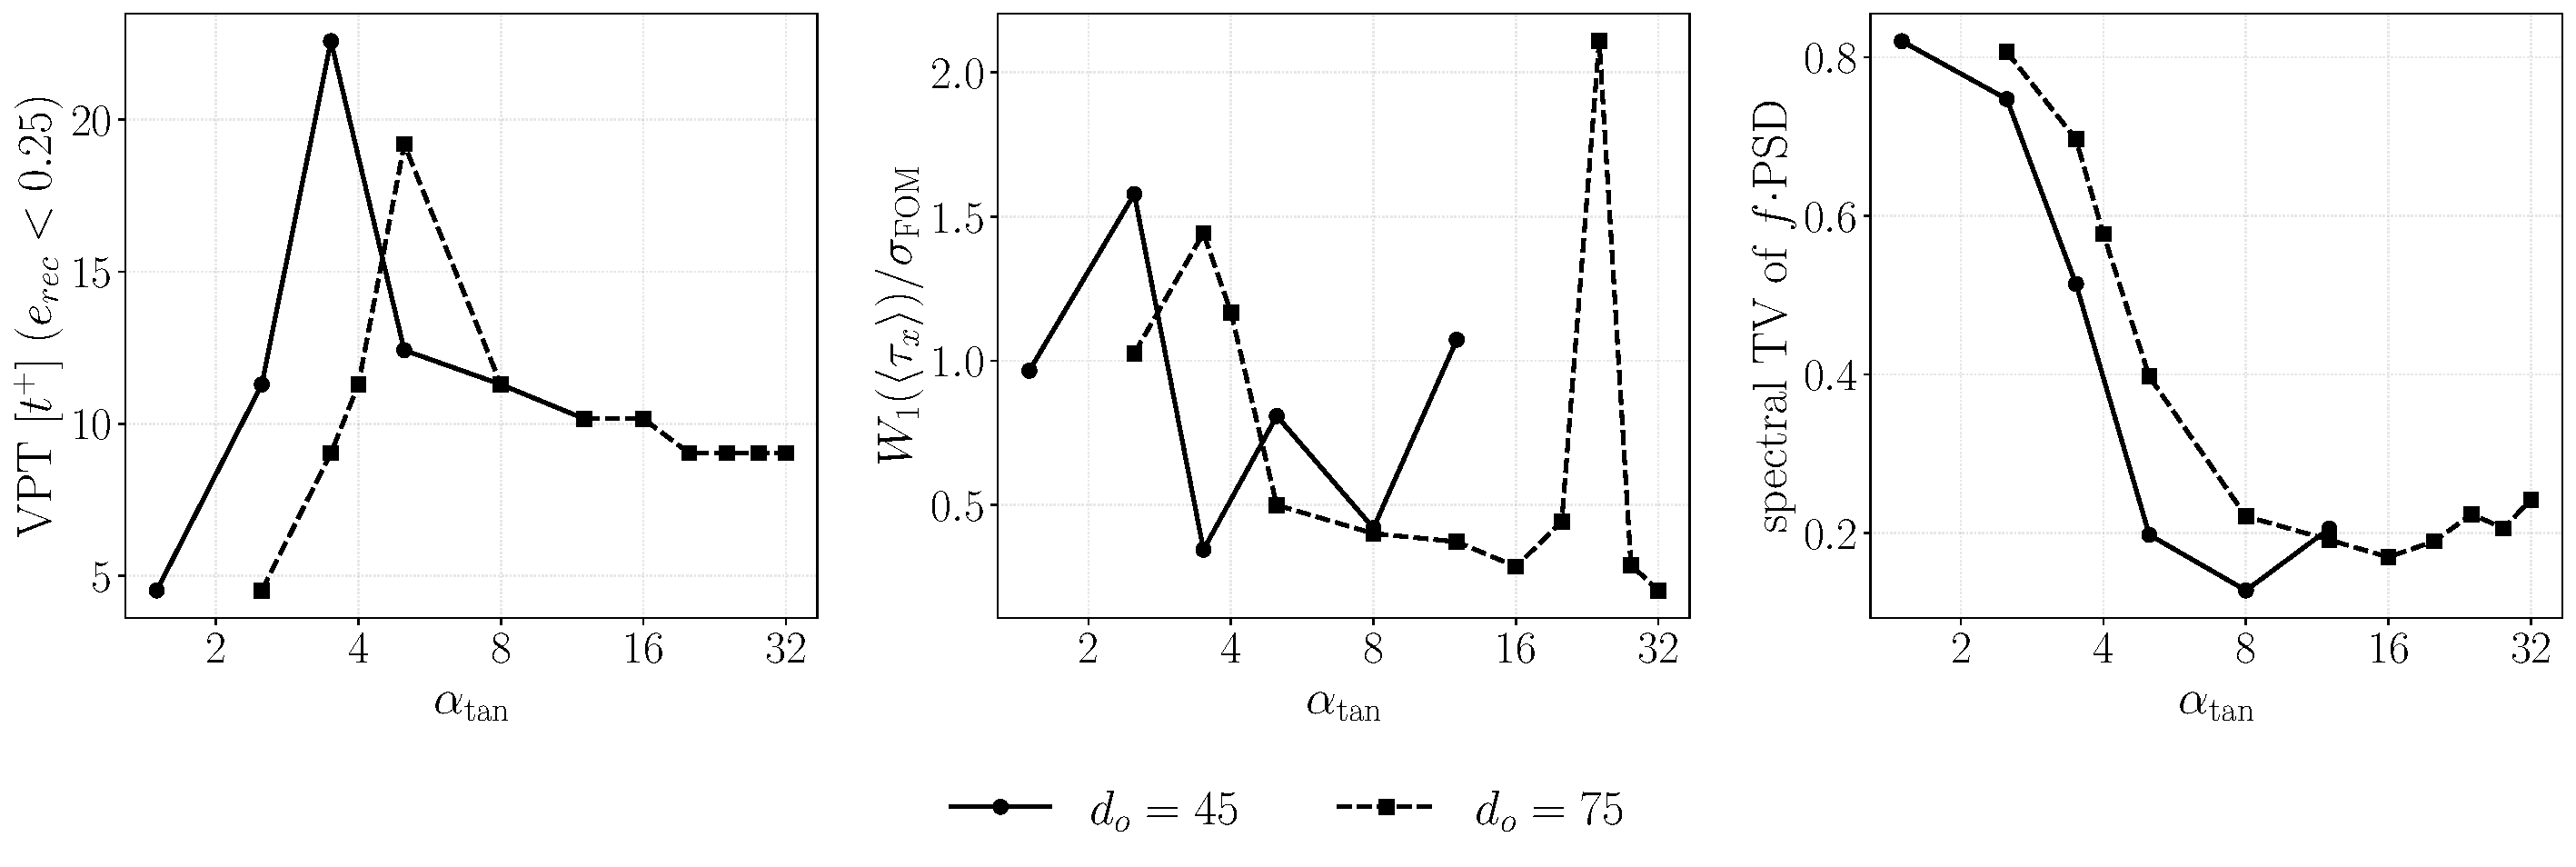
\includegraphics[width=\textwidth]{images/fig6_vpt_climate_vs_nrmse.pdf}
	\caption{Predictability and climate against anisotropy. For $d_o=45$ and $75$
	against $\alpha_{\mathrm{tan}}$: (a) valid prediction time to reconstruction error
	$e_{\mathrm{rec}}=0.25$; (b) Wasserstein-1 distance of the skin-friction
	distribution in units of $\sigma_{\mathrm{FOM}}$; (c) total-variation distance of
	the premultiplied spectrum $f\cdot\mathrm{PSD}$.}
	\label{fig:vptclimate}
\end{figure}

\begin{figure}[H]
	\centering
	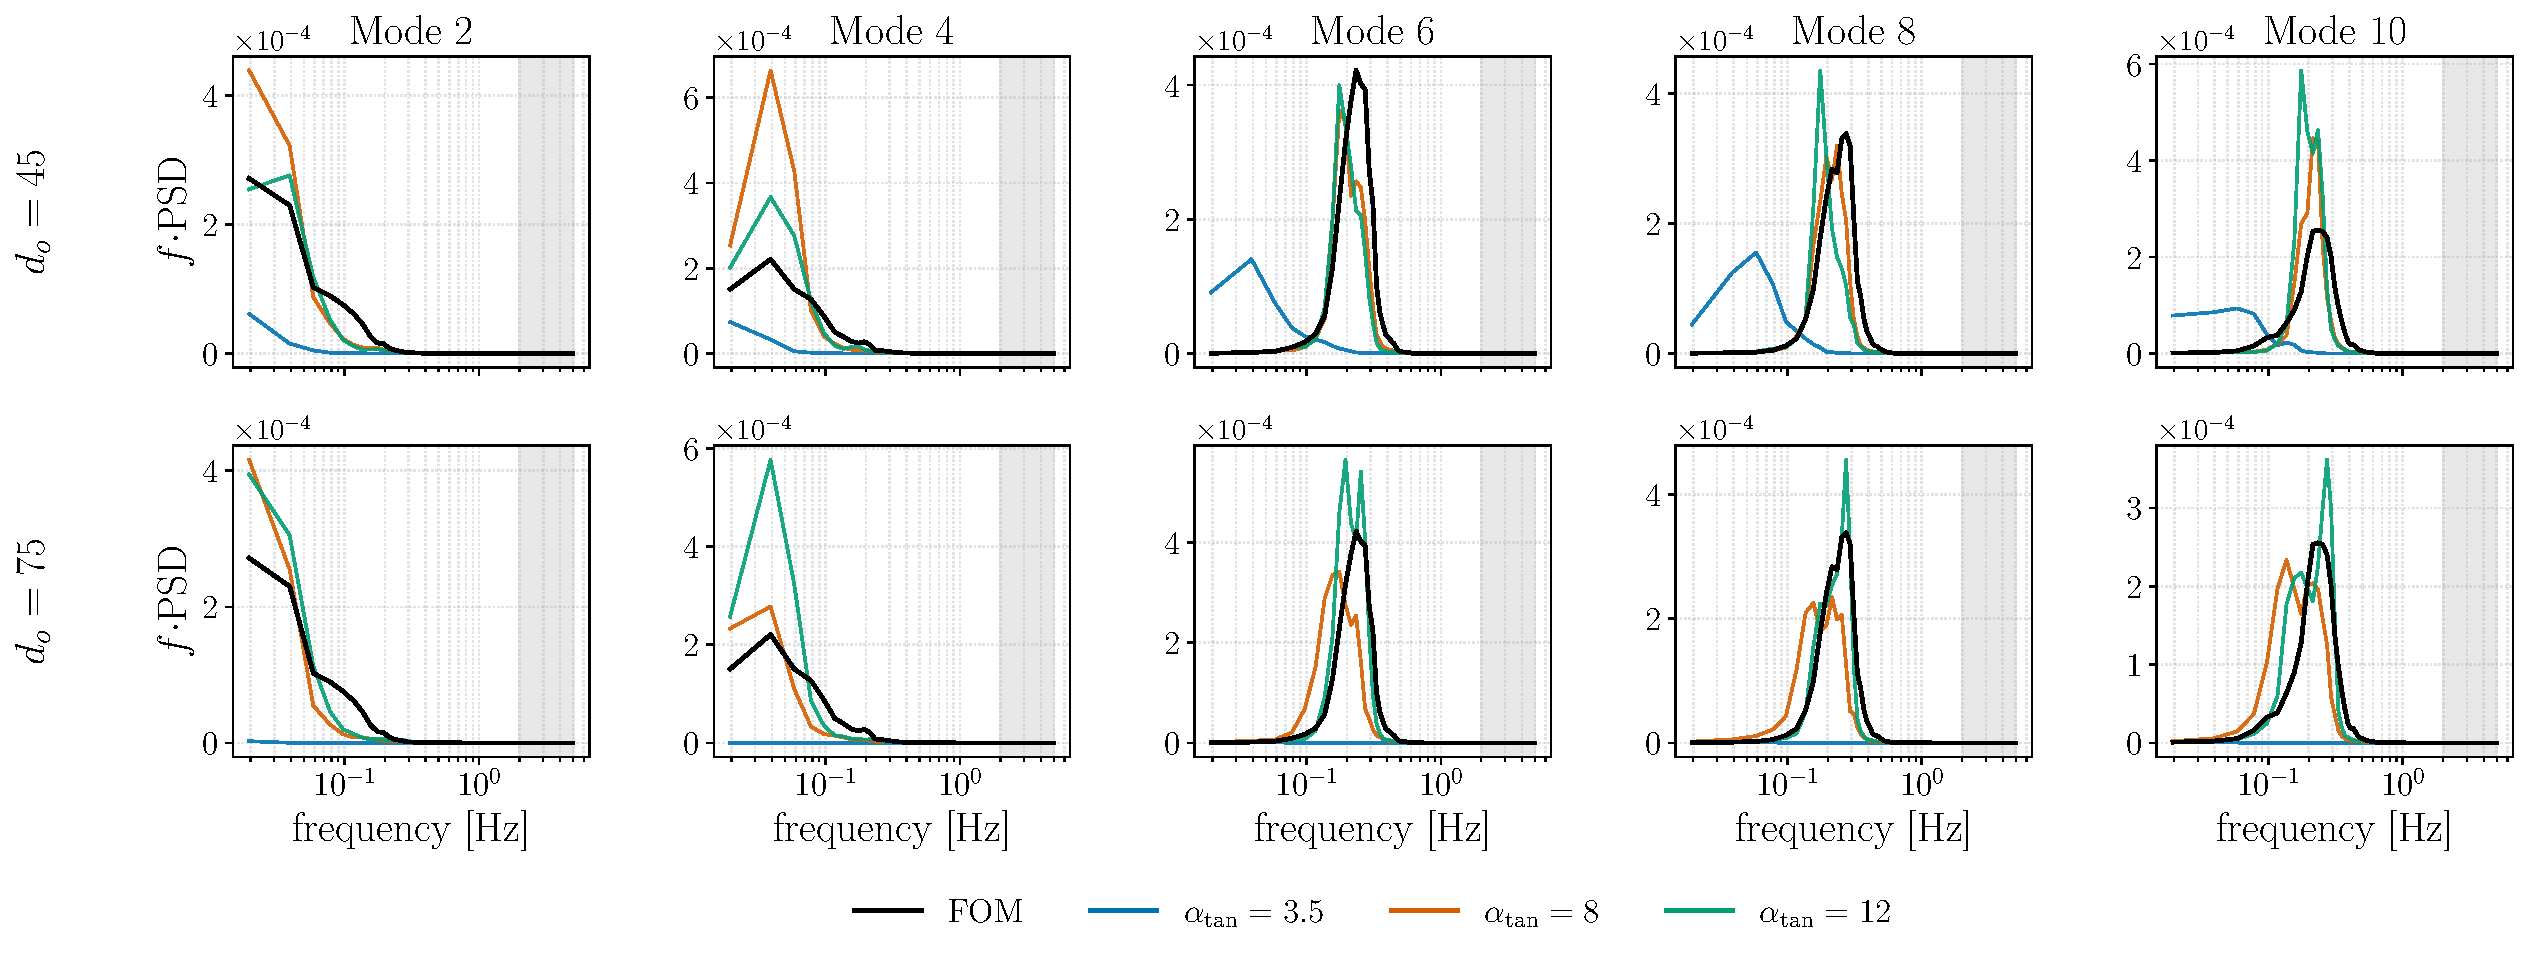
\includegraphics[width=\textwidth]{images/fig8_psd_modes.pdf}
	\caption{Spectral fidelity of the free run. Premultiplied spectra
	$f\cdot\mathrm{PSD}$ of latent modes 2, 4, 6, 8 and 10 for the free-integrated
	model at three values of $\alpha_{\mathrm{tan}}$ and the reference (FOM), for
	$d_o=45$ (top) and $75$ (bottom). Shading marks frequencies above the reference
	band limit.}
	\label{fig:psdmodes}
\end{figure}
The three indicators are read against $\alpha_{\mathrm{tan}}$ for both $d_o$ in
Fig.~\ref{fig:vptclimate}. As expected from the gap between one-step fit and closed-loop rollout,
the valid prediction time, averaged over $100$ initial conditions spaced uniformly across the
test segment, about one regeneration cycle apart (panel a), does not follow the NRMSE floor of
Fig.~\ref{fig:alphanrmse}(c): the fit keeps improving with
$\alpha_{\mathrm{tan}}$, whereas the VPT peaks at an intermediate width,
$\alpha_{\mathrm{tan}}\approx 3.5$ to $5$, and declines beyond it, in both $d_o$. The peak width
is unchanged when the error threshold is varied from $0.2$ to $0.35$, so the ranking does not
hinge on the tolerance.

The climate does not follow the VPT either. A larger $W_1$ means a wider gap from the reference
skin-friction distribution, and its minimum lies at a larger $\alpha_{\mathrm{tan}}$ than the VPT
peak (panel b); the spectral distance behaves the same way (panel c). The one-step fit, the
predictability and the long-time statistics are each optimised at a different width, so a single
global $\alpha_{\mathrm{tan}}$ trades one against another.

The origin of this trade-off is the plane average itself. It keeps only the spatial-mean part of
each mode, so $\langle\tau_x\rangle$ is
carried by a few low-order modes; the energetic streak pair, spanwise-alternating, averages to
near-zero across the span and barely contributes. At small $\alpha_{\mathrm{tan}}$ the coverage
gaps leave the fitted field unable to drive even these modes, and the free run relaxes towards a
near-fixed state, so $\langle\tau_x\rangle$ is weak (Fig.~\ref{fig:skinfriction}). As the width
grows the modes regain their motion, but around $\alpha_{\mathrm{tan}}\approx 3.5$ to $5$ the
active low-order modes oscillate more slowly than the reference (Fig.~\ref{fig:psdmodes}), so the
reconstructed $\langle\tau_x\rangle$ is red-shifted rather than lacking its faster content.
\begin{figure}[H]
	\centering
	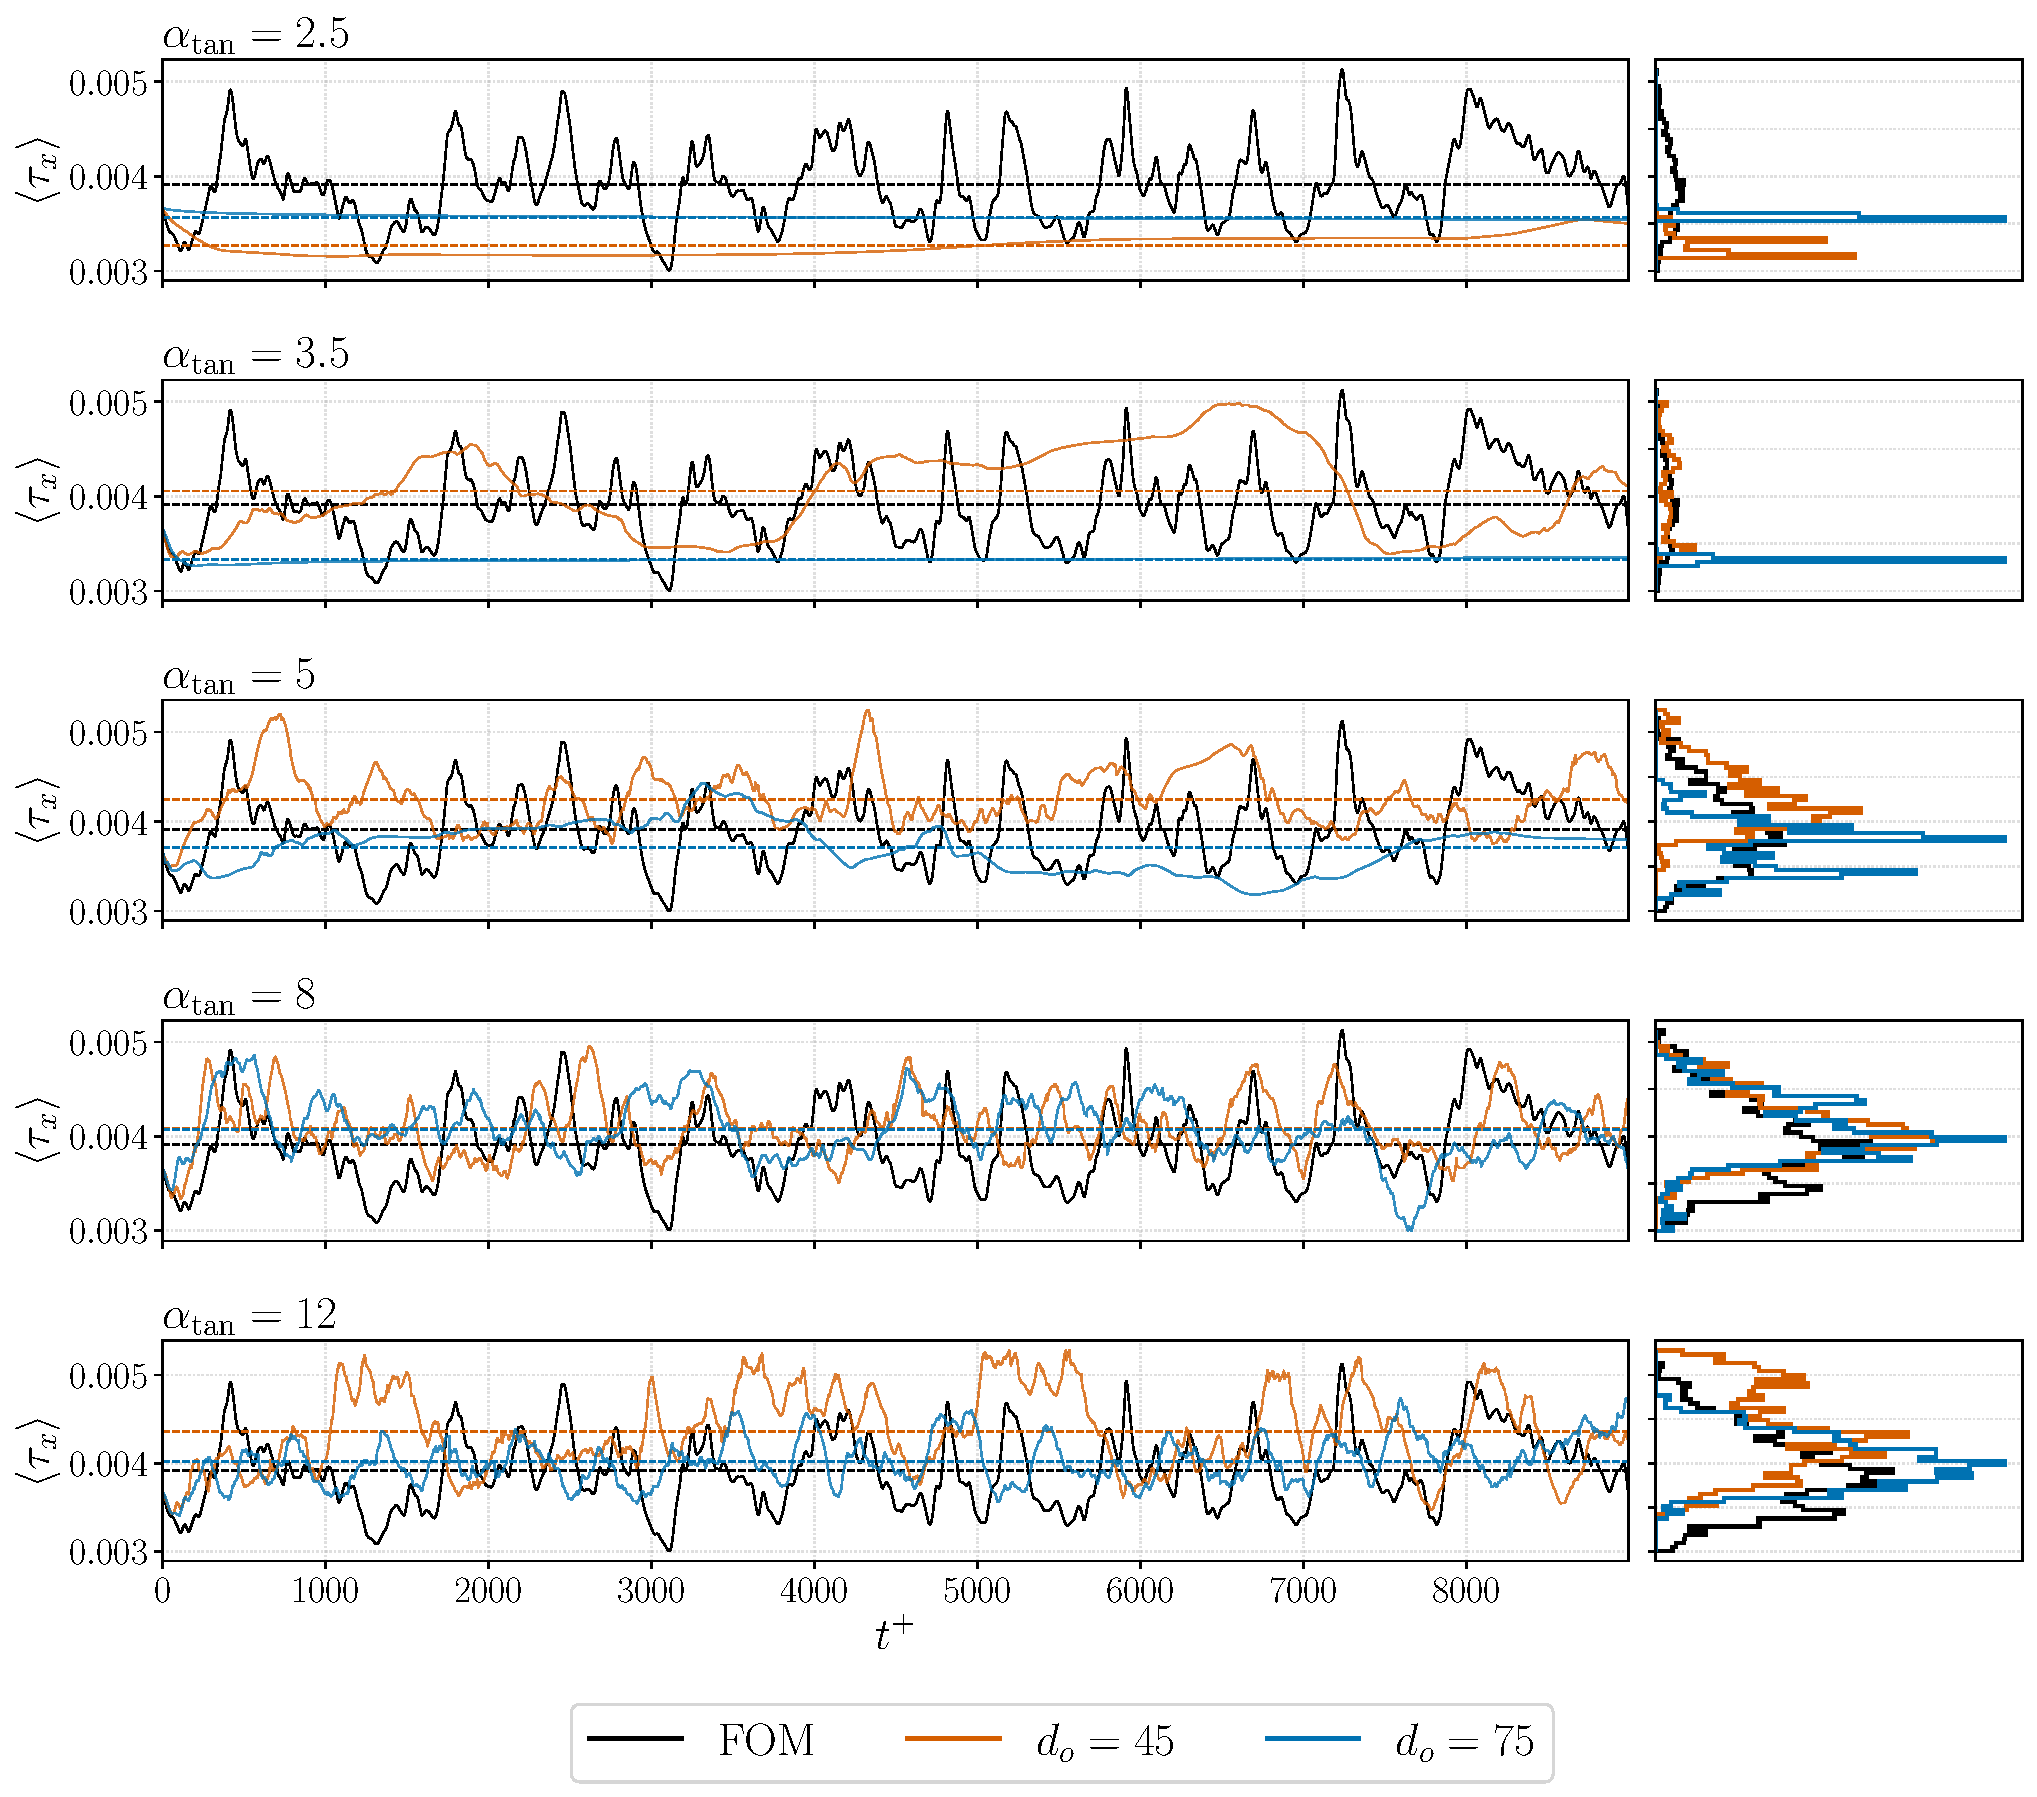
\includegraphics[width=\textwidth]{images/fig7_skin_friction_alpha_grid.pdf}
	\caption{Free-running skin friction. Spatially averaged streamwise wall shear
	$\langle\tau_x\rangle$ against time for the free-integrated model at $d_o=45$
	and $75$ and the reference (FOM), one row per $\alpha_{\mathrm{tan}}$, with the
	time means dashed. Right: the marginal distributions.}
	\label{fig:skinfriction}
\end{figure}

The climate, by contrast, sharpens at larger widths, the friction and spectral distances reaching
their lowest values around $\alpha_{\mathrm{tan}}\approx 8$ to $16$. Wider, more strongly
overlapping kernels smooth the fitted field: this costs local accuracy, and so predictability,
but favours a bounded, correctly occupied long-time state, reminiscent of the trade of short-term
accuracy for long-time stability seen when dissipation is added to POD--Galerkin models
\citep{Aubry_Holmes_Lumley_Stone_1988,rempfer2000low}, here a by-product of the wider kernels
rather than an explicit dissipation.

The higher truncation does not shift this: on all three measures $d_o=75$ is no better than
$d_o=45$. The modes added between the two are already inert for the skin-friction statistics targeted here,
and this is the evidence for not fitting the still smaller-scale tail up to $d_o=170$: more of
that incoherent content adds reconstruction accuracy without enriching the dynamics.

These trade-offs set the operating point. A wall-only model is asked to carry the cycle's
statistics rather than a single trajectory, so the width is chosen for the invariant measure: the
model is run at $d_o=45$ and $\alpha_{\mathrm{tan}}=8$, the low end of the range where the friction
distribution and the spectrum are closest to the reference, kept near the predictability peak, at
the cost of a shorter prediction horizon than the width that maximises it. At this setting the free run reproduces the
skin-friction distribution and premultiplied spectrum of the direct simulation
(Fig.~\ref{fig:skinfriction}, Fig.~\ref{fig:psdmodes}). The wall-shear field, integrated on its
own, sustains the near-wall cycle's statistics.

\section{Reading the near-wall cycle from the fitted field}\label{sec:interp}

The same field that sustains these statistics is explicit and differentiable, so it can be read
as a dynamical system rather than only run forward: its resting states, its Jacobian,
and the growth of small perturbations are all available in closed form. This is what the
present section exercises; it closes on the limit of what the wall state can determine.

Since the field $\dot{\bfa}=f(\bfa)$ is defined over the whole attractor, its slow points
can be located directly. A slow point is a state at which the model's tendency vanishes,
an equilibrium of the fitted field near which the flow moves slowly. The local dynamics
there are unstable (Section~\ref{sec:dynstates}), so these are weakly unstable
near-equilibria. 

Solving $f(\bfa)=0$ for the production model, every recovered slow point lies in the quiescent half
of the cycle ($\sigma_y<0$), spread across streak amplitude, reminiscent of the lower- and
upper-branch family of invariant solutions of wall-bounded shear flow
\citep{nagata1990three,waleffe2001exact,tohitano2003periodic}
(Fig.~\ref{fig:slowpoints}). The roots sit well within the sampled data, where the
corrector never acts, so they are not artefacts of thin kernel coverage.

The same holds across four independently fitted models, whose escape-time distributions
agree (Fig.~\ref{fig:slowpoints}b). The cycle's rhythm is asymmetric: the quiescent phase
offers weakly unstable anchors the flow lingers near for tens of $t^+$, while the active
phase holds nothing and is crossed quickly. The near-wall cycle's unstable invariant
solutions show the same rhythm, shadowed between fast bursts
\citep{kawahara2001periodic,kawahara2012significance}; these slow points of the wall-visible
mean are not those solutions, nor equilibria of the flow, which has none.

\begin{figure}[H]
	\centering
	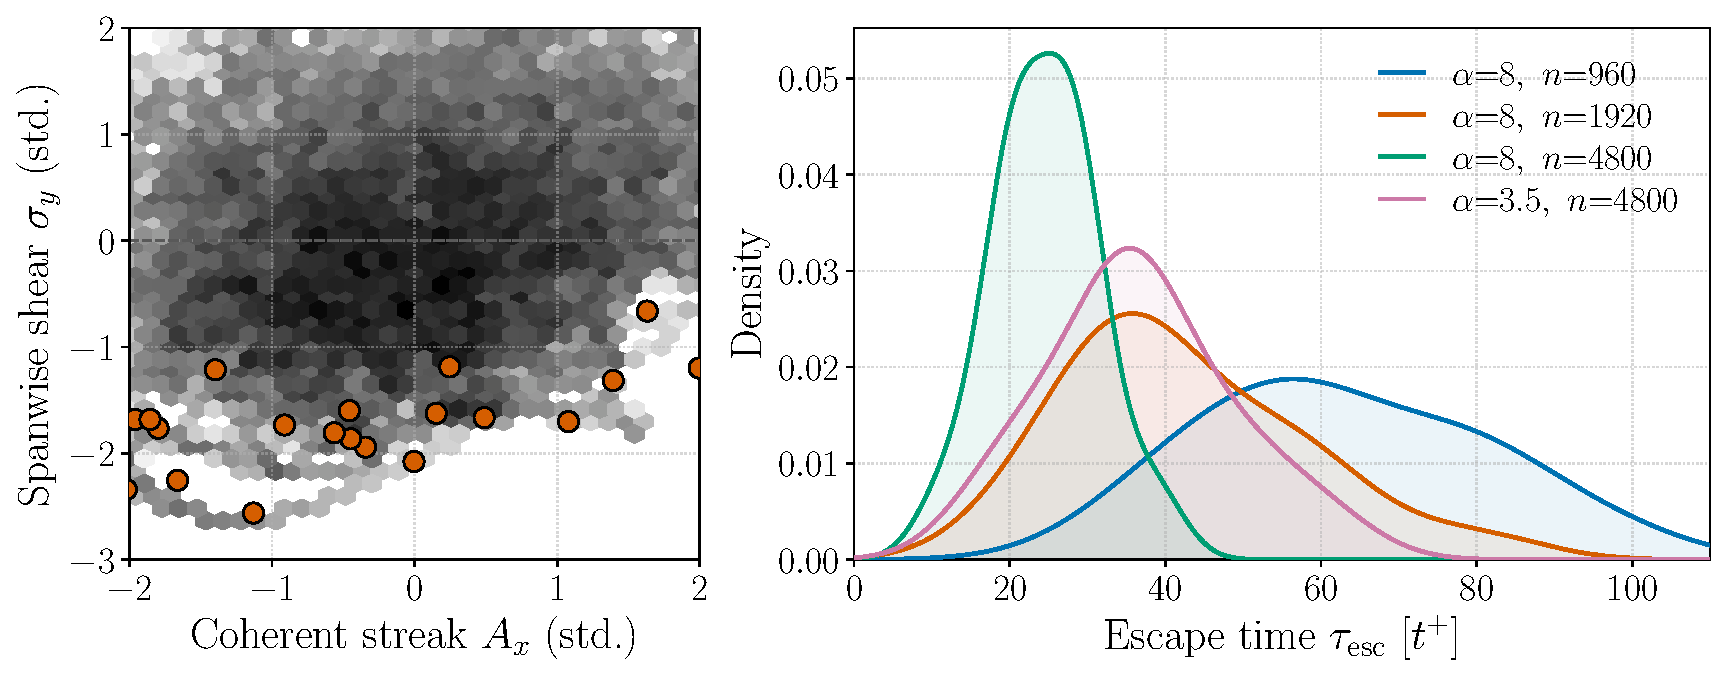
\includegraphics[width=\textwidth]{images/fig14_slowpoints.pdf}
	\caption{Slow points live only in the quiescent phase. (a) States at which the fitted
	field's mean tendency vanishes, for the production model
	($\alpha_{\mathrm{tan}}=8$, $1920$ kernels), on the streak--vortex plane over
	the sampled density (grey); all lie in the quiescent half ($\sigma_y<0$), the
	active half none. (b) Escape-time distribution of the slow points for four
	independently fitted models, varying $\alpha_{\mathrm{tan}}$ and kernel count
	$n$: tens of $t^+$ in every case.}
	\label{fig:slowpoints}
\end{figure}

The slow points say where the flow rests; the Jacobian says how nearby trajectories are
stretched and squeezed. Differentiating the field gives $J=\partial f/\partial\bfa$, and
linearising it reads off the local anatomy of the cycle (Fig.~\ref{fig:anatomy}). Beyond the
eigenvalues that separated the phases in Section~\ref{sec:dynstates}, its non-normality
measures the worst-case transient amplification of a disturbance over a short horizon, and its
trace whether a cloud of nearby states contracts.

The non-normal growth asks how sensitive the flow is to perturbations. Over a $10\,t^+$ horizon,
$G$ is the largest factor by which a small disturbance grows in the latent-coefficient
energy norm, the leading singular value of the tangent-linear propagator integrated
along the trajectory rather than frozen at a point
\citep{schmid2007nonmodal,trefethen1993hydrodynamic}. Built this way, it captures the
transient amplification a non-normal field allows even where the eigenvalues decay
\citep{butler1992optimal}. A large $G$ marks a sensitive phase, where a small difference
grows fast; read per cluster (Fig.~\ref{fig:anatomy}a), it peaks at burst onset, where a
nudge grows about $2.5$-fold. This is the growth in the wall-visible coordinates alone,
and the latent norm is not the physical energy, so $G$ is a wall-projected proxy for the
full growth rather than a bound on it.

The trace of $J$ looks at a whole cloud of nearby states rather than a single disturbance, and
indicates the rate at which a small volume of states contracts or grows. As shown in
Fig.~\ref{fig:anatomy}a, the squeezing is hardest deep in the burst and slackens to almost
nothing at burst onset. The sign of $\mathrm{tr}\,J$ there varies between fits, so only the
ordering is read, and it is the contraction of the wall-visible latent volume, not the flow's
own dissipation.

Placed on the cycle of Section~\ref{sec:dynstates}, the most amplifying phase is the mature
streak (Q1): the streak is at its most fragile just as it reaches full strength, on the point
of breaking down. The quiescent state (Q3) is the least sensitive of all. The
strongest contraction sits in the breakdown itself, spanning the late streak and the
vortex-dominated phase, where the disturbances the streak has amplified are dissipated as it
comes apart.

\begin{figure}[H]
	\centering
	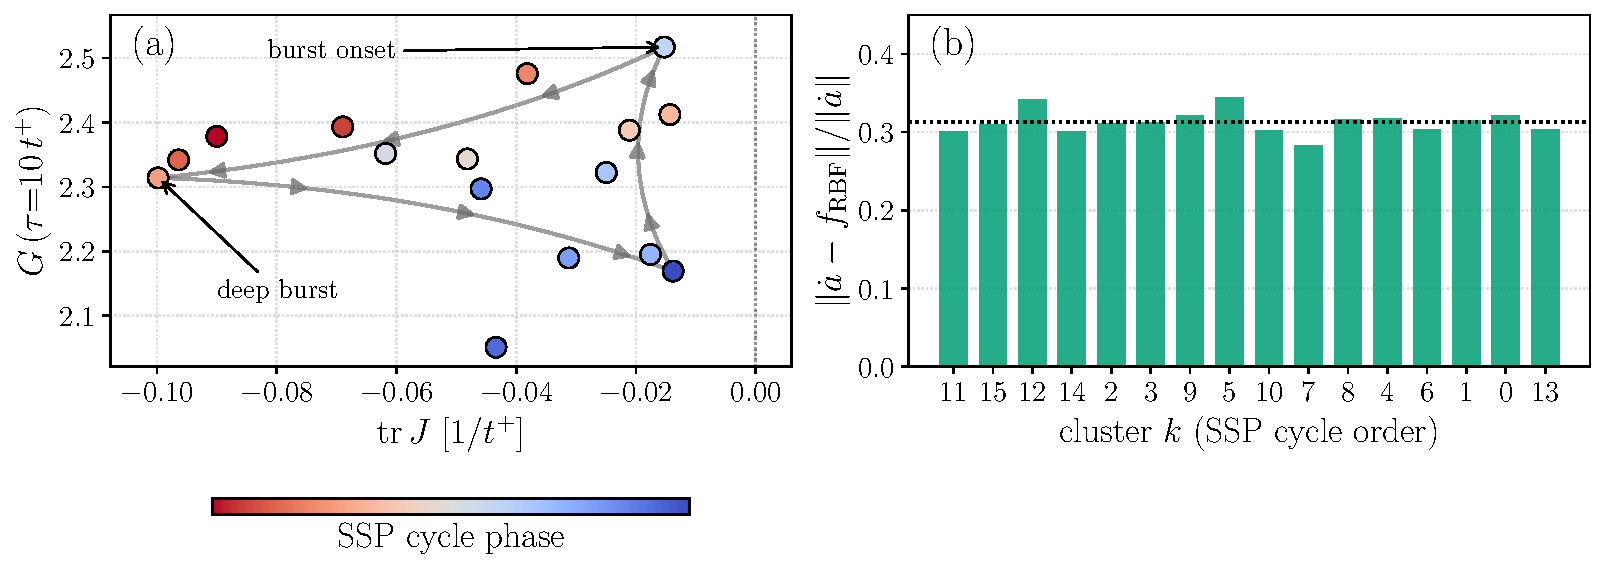
\includegraphics[width=\textwidth]{images/fig15_anatomy.pdf}
	\caption{Dynamical anatomy of the cycle, read off the fitted field. (a)
	Non-normal growth $G$, the worst-case amplification over a $10\,t^+$ horizon,
	against phase-volume contraction $\mathrm{tr}\,J$, one point per cluster,
	coloured by cycle phase. Burst onset is least contracting and most amplifying
	(upper right), the deep burst most contracting; $G$ is the wall-visible
	amplification, reported against the field's modal and numerical-abscissa bounds,
	and $\mathrm{tr}\,J$ is the mid of the four-fit range. (b) Closure deficit
	per cluster: the fraction of the wall tendency not determined by the wall state,
	near $0.3$ and phase-uniform.}
	\label{fig:anatomy}
\end{figure}

The readings so far are what the wall field reveals; one number bounds what it cannot determine
(Fig.~\ref{fig:anatomy}b). About $30\%$ of the instantaneous wall tendency cannot
be written as a function of the wall state, the same in every phase. This is the share of what
happens next that the wall cannot know from what it sees now, set by the interior motions it
does not observe, and it is why the model holds the climate but not the trajectory. The next
section measures what this one-step deficit accumulates to over the assimilation window, in
inflation units.

\section{Data assimilation and wall-observable autonomy}\label{sec:enkf}

The free run of Section~\ref{sec:recover} reproduces the cycle's statistics, and
with them its invariant measure. The near-wall region sustains its cycle when the
motions above the buffer layer are quenched \citep{jimenez1999autonomous}, which
justifies a low-dimensional model of it; whether the wall shear, a two-component
footprint of that three-dimensional cycle, is a sufficient coordinate for it is a
separate question. That the climate is correct does not mean the instantaneous wall
shear fixes what the cycle does next.

The cycle turns on the buffer-layer state above the wall: the wall-normal velocity
that drives the lift-up, and the streamwise vortices that regenerate the streaks
\citep{Waleffe_1997,Hamilton_Kim_Waleffe_1995}. The wall carries only their
footprint, so a field fitted in wall coordinates learns a conditional-mean tendency
\citep{chorin2000optimal}, averaged over the interior motions it does not see. Section~\ref{sec:interp} read
this off as a closure deficit at a single step; what follows measures the forecast
error it produces over short windows, the cost the wall-only model pays for the
events off the wall.

Data assimilation is the natural tool: the wall shear is what an experiment can
measure, even with sparse and noisy sensors, and the forecast is corrected online,
without re-solving the model or forming an adjoint, so it is cheap. Assimilating
wall measurements into a flow model has precedent with the governing equations in
the loop \citep{colburn2011state} and with a data-driven reduced model in their
place \citep{ozalp2026realtime}. The estimator is a Kalman filter, alternating a
forecast, in which the model advances the state and its uncertainty, and an
analysis, in which the forecast is pulled towards the observations, the two weighted
by their covariances through the Kalman gain \citep{kalman1960new}.

The classical filter propagates the full covariance through the linearised dynamics.
To avoid the linearisation, an ensemble Kalman filter (EnKF) carries a Monte Carlo
ensemble, integrates each member through the nonlinear field, and reads the forecast
covariance from their spread \citep{evensen2003ensemble}. This captures the nonlinear
error growth along the attractor, at a cost that scales with the ensemble size and
the latent dimension rather than the full state.

\begin{figure}[H]
	\centering
	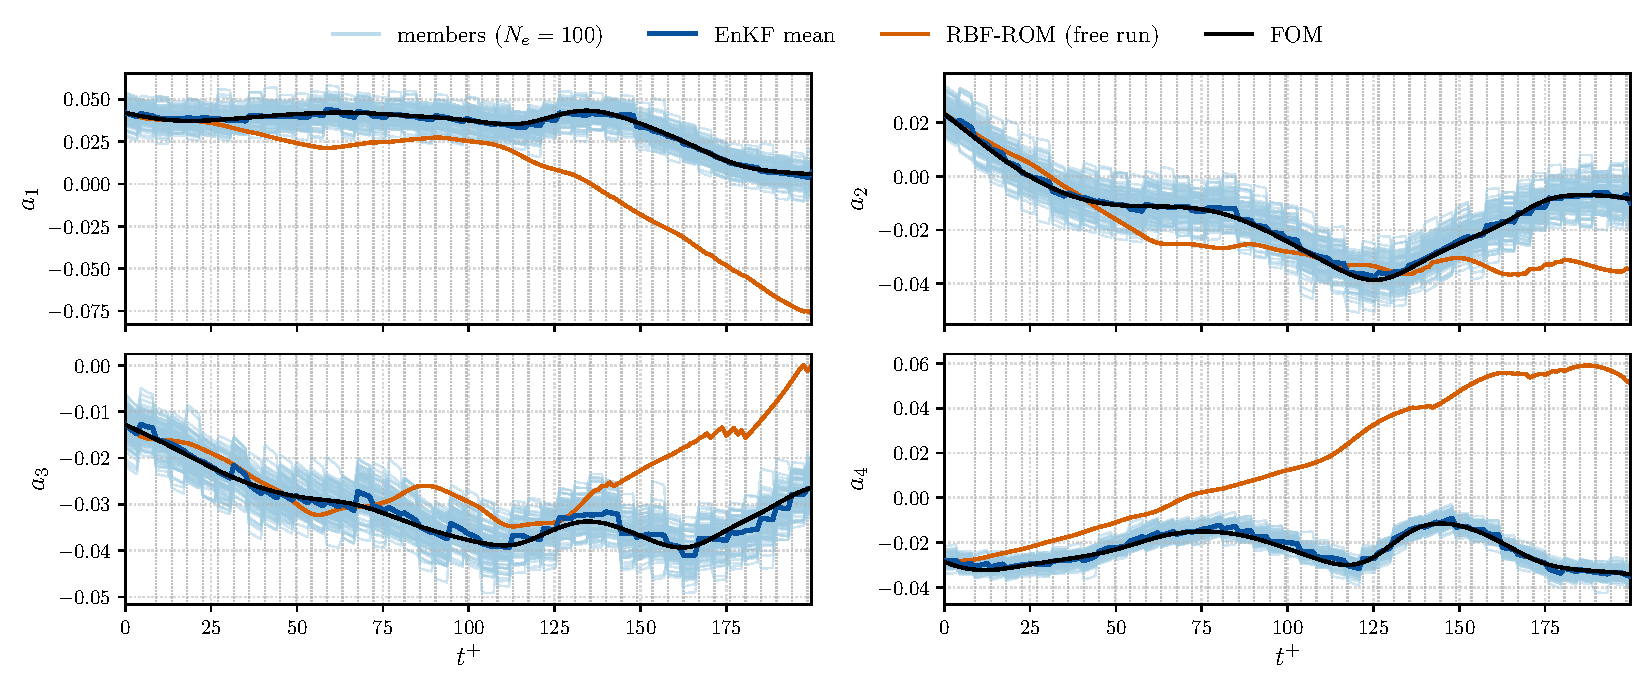
\includegraphics[width=\textwidth]{images/fig9_enkf_modes.pdf}
	\caption{Ensemble forecast of the leading modes. Latent coefficients $a_1$ to
	$a_4$ against $t^+$ for the ensemble Kalman filter ($N_e=100$ members), its
	mean, the free-running RBF-ROM and the reference (FOM). Dotted verticals mark
	the analysis times.}
	\label{fig:enkfmodes}
\end{figure}

The filter runs on the reduced coordinates, observing the two wall-shear components
on a uniform grid of stride $\Delta$, so $N_{\mathrm{obs}}=2(64/\Delta)^2$ per
sample. Each sensor carries independent Gaussian noise of standard deviation
$\sigma_{\mathrm{obs}}$ relative to the root-mean-square of the wall-shear
fluctuation, giving a diagonal observation covariance, and the observations are
perturbed per member.
\begin{table}[t]
	\centering
	\caption{Baseline data-assimilation parameters.}
	\label{tab:enkf}
	\begin{tabular}{llc}
		\toprule
		Parameter & Symbol & Value \\
		\midrule
		Ensemble size & $N_{\mathrm{ens}}$ & $100$ \\
		Sensor stride & $\Delta$ & $8$ \\
		Observed components & & $\tau_x,\tau_y$ \\
		Number of sensors & $N_{\mathrm{obs}}$ & $128$ \\
		Observation noise & $\sigma_{\mathrm{obs}}$ & $0.1$ \\
		Assimilation cadence & $\Delta t_{\mathrm{obs}}^+$ & $5$ \\
		Multiplicative inflation & & $1.02$ \\
		Additive inflation & $q$ & $0.1$ \\
		\bottomrule
	\end{tabular}
\end{table}
An ensemble of $N_{\mathrm{ens}}$ members is initialised by perturbing a snapshot
about the attractor, advanced through the fitted field between analyses, and
corrected every $\Delta t_{\mathrm{obs}}^+$. Multiplicative and additive inflation
counter ensemble collapse, the additive level $q$ being the knob examined below;
Table~\ref{tab:enkf} lists the baseline values, with the stride, noise level and
cadence varied later. On the leading modes (Fig.~\ref{fig:enkfmodes}) the ensemble
brackets the reference, and its mean tracks the true trajectory where the free run,
given the same start, drifts away.

At each analysis the filter compares the incoming observations with its own
forecast; the mismatch between the two, the innovation $d$, is the only quantity
it can weigh against its own error estimate. Scaling $d$ by the covariance
$S=\mathbf{H}\mathbf{P}^f\mathbf{H}^\top+\mathbf{R}$ it predicts for it gives the
normalised innovation squared, a measure of whether the mismatch exceeds the spread
the filter expected. Here $\mathbf{H}$ is the linear map from the reduced state to
the sensors, $\mathbf{P}^f$ the forecast covariance carried by the ensemble spread,
and $\mathbf{R}$ the diagonal observation-noise covariance.
\begin{figure}[H]
	\centering
	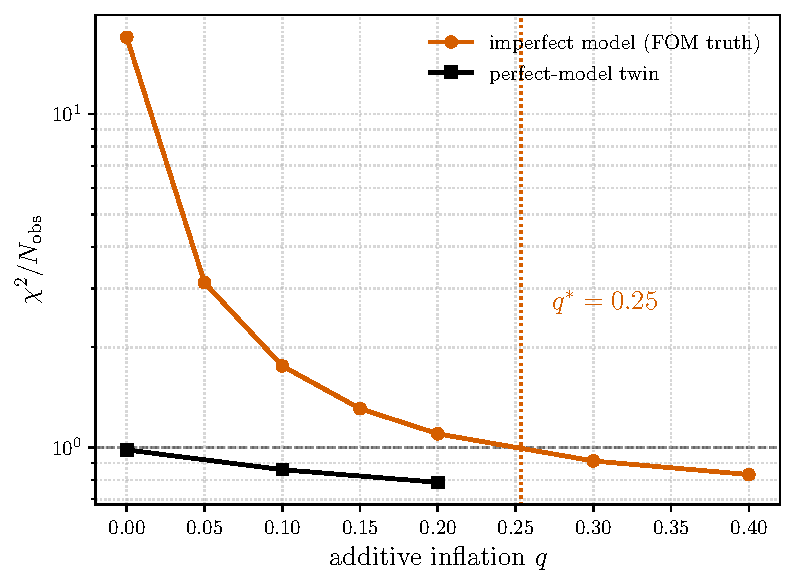
\includegraphics[width=0.62\textwidth]{images/fig10_enkf_qstar.pdf}
	\caption{The additive-inflation floor. Time-averaged $\chi^2/N_{\mathrm{obs}}$
	against the additive inflation $q$, for the model assimilating FOM observations
	and for the perfect-model twin. The crossing of $\chi^2/N_{\mathrm{obs}}=1$
	(dashed) sets $q^\ast$; the twin needs none.}
	\label{fig:enkfqstar}
\end{figure}
When the filter is consistent this statistic averages to one per observation,
$\chi^2/N_{\mathrm{obs}}=1$. This is known as the standard innovation-consistency check
\citep{desroziers2005diagnosis}. 

If the model that advances the ensemble is missing dynamics, it produces
innovations too large for the spread it predicts, so $\chi^2/N_{\mathrm{obs}}>1$.
Enlarging the forecast covariance by additive inflation $q$ restores consistency,
and the level that brings $\chi^2/N_{\mathrm{obs}}$ back to one is $q^\ast$: the
process noise the wall-only model must inject to account for its own error, the
established way of reading model error off the innovations
\citep{dee1995online,anderson2007adaptive,tandeo2020review}.

The value of $q^\ast$ carries a physical reading: it is an upper bound on the
forecast error the wall-only model incurs from the interior motions it does not
carry, in units of the attractor's climatological standard deviation.
Figure~\ref{fig:enkfqstar} locates it as the crossing of $\chi^2/N_{\mathrm{obs}}=1$.
A perfect-model twin, whose truth is generated by the model itself, needs none: its
$q^\ast$ is zero, so the floor measured against the true flow is model error and not
an artefact of the filter. For the baseline configuration $q^\ast=0.25$: over each
$5\,t^+$ interval the model must inject process noise of amplitude one-quarter of the
climatological standard deviation, a few per cent of the climatological variance, to
stay statistically consistent with the observations.
\begin{figure}[H]
	\centering
	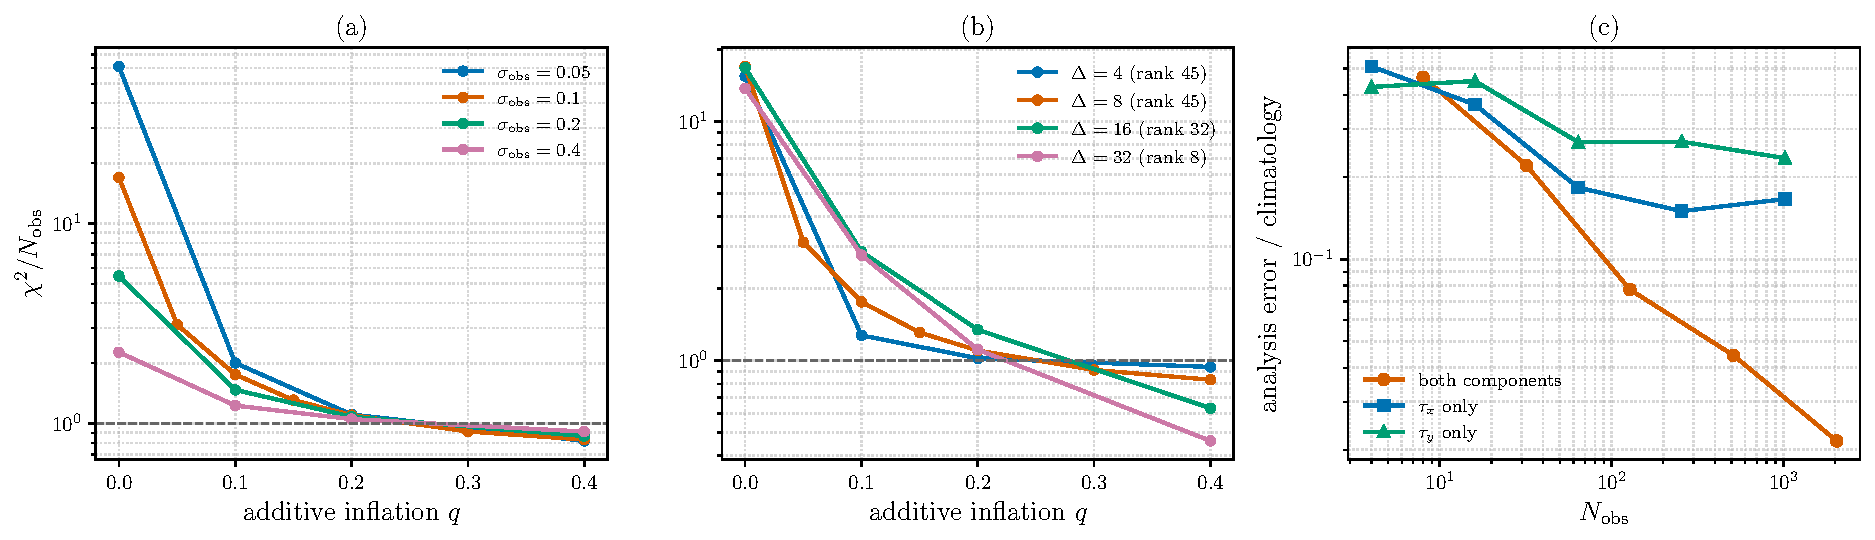
\includegraphics[width=\textwidth]{images/fig11_enkf_robustness.pdf}
	\caption{$q^\ast$ is a property of the model. $\chi^2/N_{\mathrm{obs}}$ against
	$q$ across (a) observation-noise level $\sigma_{\mathrm{obs}}$ and (b) sensor
	stride $\Delta$ (rank of $H$ in the legend); the unit crossing barely moves.
	(c) Analysis error, normalised by climatology, against sensor count
	$N_{\mathrm{obs}}$ for $\tau_x$, $\tau_y$ and both components.}
	\label{fig:enkfrobust}
\end{figure}

To separate the model-error floor from the way the wall is observed, $q^\ast$ is
measured across the measurement configuration: the observation-noise level and the
sensor stride (Fig.~\ref{fig:enkfrobust}). Over an eightfold range of noise (a) and
of stride (b), the crossing of $\chi^2/N_{\mathrm{obs}}=1$ barely moves, holding near
$q^\ast\approx0.25$. Raising the noise only lowers the curve at $q=0$, since a larger
$\mathbf{R}$ makes the same innovations less surprising, and leaves the crossing where
it was. The stride is more severe: at $\Delta=32$ the wall resolves only 8 of the 45
modes, the rank of $\mathbf{H}$ in the legend, yet $q^\ast$ is unchanged. The floor is
therefore a property of the model, not of the filter or the sensing, which is what
lets it be read as the model's own error.

The state estimate itself does depend on the sensing. Panel (c) shows the analysis
error, normalised by the climatological spread, falling as sensors are added; both
shear components together beat either alone, and $\tau_x$ carries more than $\tau_y$,
the streaks leaving a stronger streamwise footprint than the quasi-streamwise vortices
leave in the spanwise shear. Denser, two-component sensing thus sharpens the estimate
without moving the floor: how well the wall is read and how much the wall omits are
separate quantities.


\begin{figure}[H]
	\centering
	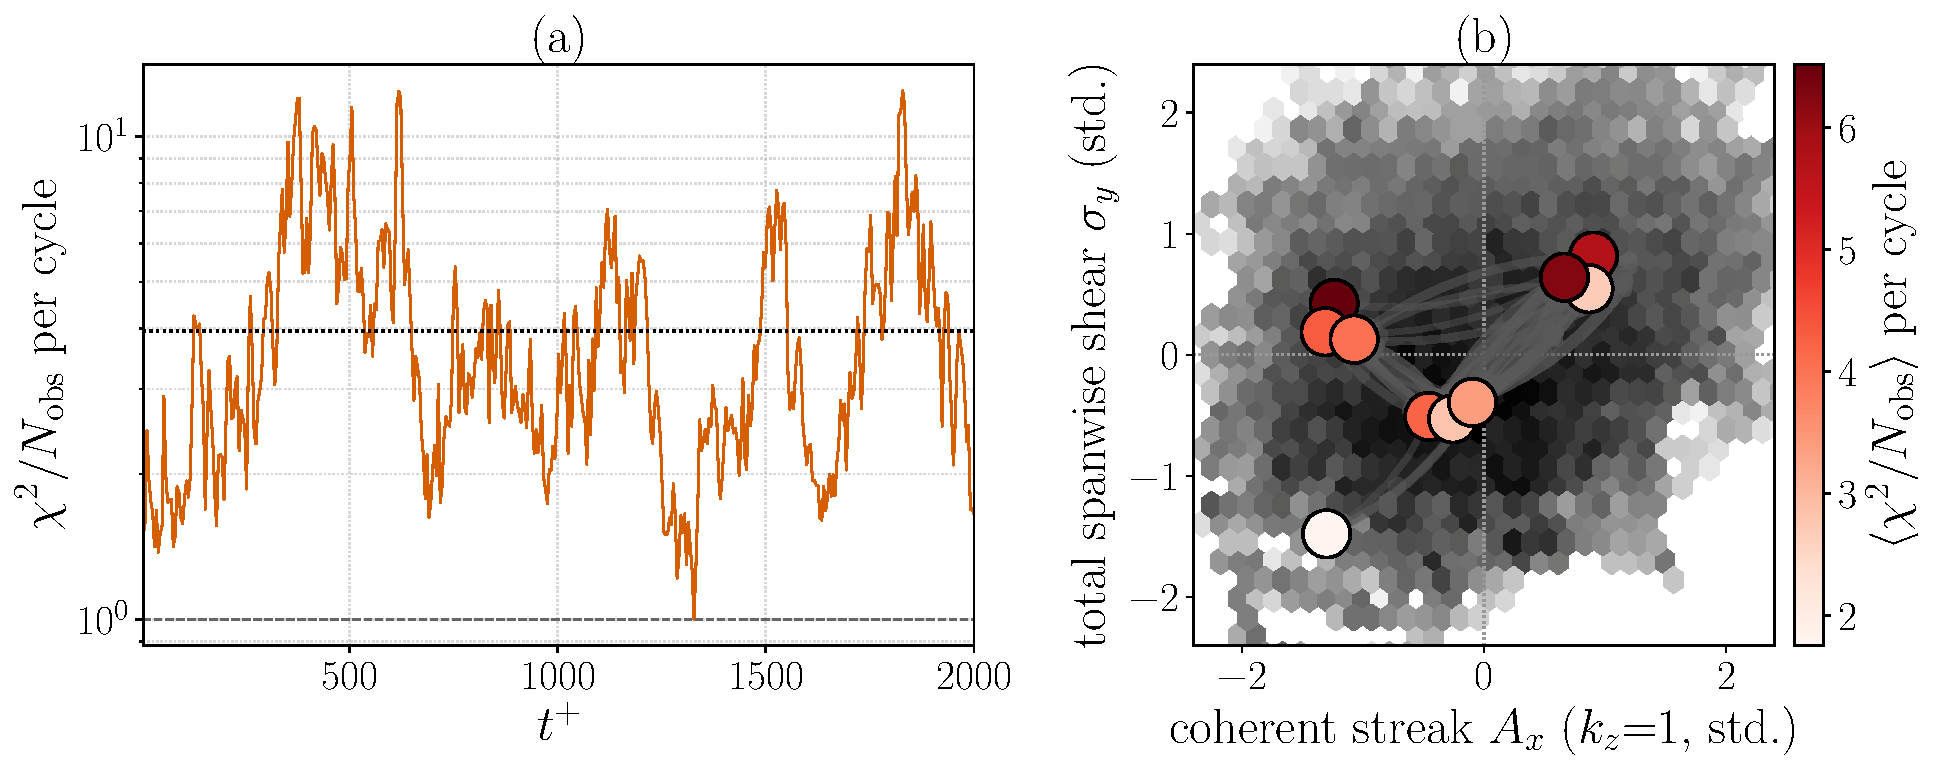
\includegraphics[width=\textwidth]{images/fig12_enkf_cadence_bursts.pdf}
	\caption{Innovation consistency in time and around the cycle. (a) Per-cycle
	$\chi^2/N_{\mathrm{obs}}$ over a $2000\,t^+$ run; the cycle mean (dotted) sits
	above consistency (dashed), the excess arriving in bursts. (b) The same
	statistic cycle-averaged per cluster, on the streak--vortex plane over the
	sampled density (grey) and coloured by $\langle\chi^2/N_{\mathrm{obs}}\rangle$;
	it is larger in the active, high-$\sigma_y$ phase and near-consistent in the
	quiescent phase, tracing the cycle (faint arrows).}
	\label{fig:enkfcadence}
\end{figure}
The floor $q^\ast$ is a time average, and resolved along the run it is not uniform.
As shown in Fig.~\ref{fig:enkfcadence}a, the per-cycle $\chi^2/N_{\mathrm{obs}}$ 
is bursty and the excess arrives in bursts. When mapped per cluster along the 
cycle and streak and spanwise wall shear metrics, the innovation is
largest in the active half  (Fig.~\ref{fig:enkfcadence}b), spanning the mature 
streak and its breakdown. However, on the quiescent phase the average reduced significantly.

This excess
is genuine forecast error rather than ensemble under-dispersion: the realised error is
larger in the active phase while the spread stays flat across the cycle, and it scales
with the cycle phase, not the state amplitude. 

The one-step closure deficit of
Section~\ref{sec:interp} is phase-uniform, so this localisation is a matter of its
integration: the fitted field amplifies a perturbation most in the same active phase,
where the interior motions the wall cannot resolve, the lift-up and the streak
breakdown that regenerates the vortices, are also strongest. The model's missing
information is thus concentrated in the phase where the cycle is driven from off the
wall.

\section{Conclusions}\label{sec:conclusions}

The near-wall self-sustaining cycle has been reduced to a differentiable latent field
fitted from wall shear stress alone. Resampling the trajectory in arc length and
clustering under a local Mahalanobis metric align the basis with the attractor's
geometry rather than the variance hierarchy of the decomposition, and under this
geometry the mature-streak, breakdown and quiescent phases separate into sharp
populations without physical labels. Integrated freely, the model stays bounded and
reproduces the cycle's statistics and its invariant measure, the climate and not any
single orbit upon it.

Since the fitted field is explicit and differentiable, it can be read as a dynamical
system. Its slow points are located by Newton iteration and lie in the quiescent
phase, weakly unstable near-equilibria reminiscent of the cycle's lower- and
upper-branch invariant solutions. Its Jacobian resolves the anatomy of the cycle by
phase: the non-normal growth of a disturbance peaks as the streak reaches full strength
and breaks down, and the phase-volume contraction is strongest in the breakdown itself.
These readings come directly from the fitted coefficients, without recourse to the
governing equations.

Assimilating wall measurements into the model quantifies how far the wall determines
the cycle. The wall-only model reproduces the climate but not the instantaneous
trajectory: an additive-inflation floor of about a quarter of the climatological
standard deviation, stable across the sensor noise and spacing, measures the forecast
error it incurs from the interior motions it does not carry. This deficit is a fixed
fraction of the tendency at each step and concentrates, once integrated, in the active
phase where the lift-up and the streak breakdown are governed from off the wall. A
field fitted in wall coordinates therefore learns a conditional-mean tendency, and
these results are for a single friction Reynolds number in a minimal channel.

Several directions follow. The interior-information deficit invites a closure model
that injects the unresolved off-wall dynamics to lower the floor and extend the horizon
over which the wall-only forecast stays reliable. Raising the friction Reynolds number
and enlarging the domain would test whether the wall stays a near-sufficient coordinate
once the near-wall cycle is no longer isolated, and adding wall pressure to the shear
would close more of the deficit at source. With sparse, noisy wall sensors the
estimator already tracks the true trajectory, so the same construction feeds the
near-wall control strategies that the problem began with.

\bibliography{references}

\end{document}
